\documentclass[a4paper, openany]{memoir}

\usepackage[utf8]{inputenc}
\usepackage[T1]{fontenc} 
\usepackage[english]{babel}

\usepackage{fancyhdr}
\usepackage{float}

\usepackage{amsmath}
\usepackage{amsthm}
\usepackage{amssymb}
\usepackage{enumitem}
\usepackage{multicol}
\usepackage[bookmarksopen=true,bookmarksopenlevel=2]{hyperref}
\usepackage{tikz}
\usepackage{indentfirst}

\pagestyle{fancy}
\fancyhf{}
\fancyhead[LE]{\leftmark}
\fancyhead[RO]{\rightmark}
\fancyhead[RE, LO]{3H Algebra}
\fancyfoot[LE, RO]{\thepage}
\fancyfoot[RE, LO]{Pete Gautam}

\renewcommand{\headrulewidth}{1.5pt}

\theoremstyle{definition}
\newtheorem{definition}{Definition}[section]

\theoremstyle{plain}
\newtheorem{theorem}[definition]{Theorem}
\newtheorem{lemma}[definition]{Lemma}
\newtheorem{proposition}[definition]{Proposition}
\newtheorem{corollary}[definition]{Corollary}
\newtheorem{example}[definition]{Example}

\chapterstyle{thatcher}

\begin{document}

\chapter{Group Theory}
\section{Groups and Subgroups}
\subsection{Groups}
We will start by reviewing the definition of a group.
\begin{definition}
A \emph{group} is a pair $(G, \circ)$\sidefootnote{When the operation is clear, we denote the group just by the set.}, where $G$ is a set and $\circ: G \times G \to G$ is a binary operation\sidefootnote{Sometimes, we refer to this as another axiom, called \emph{closure}.} on $G$ such that:
\begin{itemize}
    \item $\circ$ is an \emph{associative} operation, i.e. for all $g_1, g_2, g_3 \in G$, $g_1 \circ (g_2 \circ g_3) = (g_1 \circ g_2) \circ g_3$;
    \item there exists an \emph{identity} element $e \in G$ such that for all $g \in G$, $g \circ e = g = e \circ g$; and
    \item for every $g \in G$, there exists an \emph{inverse} element $g' \in G$ such that $g \circ g' = e = g' \circ g$.
\end{itemize}
\end{definition}
For the third axiom of inverse to be well-defined, we require the identity element $e$ in any group to be unique. This turns out to be true, as we show below.
\begin{proposition}
Let $G$ be a group, and let $e_1, e_2 \in G$ be identity elements. Then, $e_1 = e_2$.
\end{proposition}
\begin{proof}
Consider the product $e_1 \circ e_2$. Since $e_1$ is an identity element, we find that $e_1 \circ e_2 = e_2$. Moreover, since $e_2$ is an identity element, we have that $e_1 \circ e_2 = e_1$. This implies that $e_1 = e_2$.
\end{proof}
\noindent Therefore, if the identity element exists in a group, then it is unique. By definition, a group has an identity element. So, that element must be unique.

It also turns out that the inverse of an element is unique.
\begin{proposition}
Let $G$ be a group, and let $g \in G$, and let $h_1, h_2 \in G$ be inverses of $G$. Then, $h_1 = h_2$.
\end{proposition}
\begin{proof}
We find that
\begin{align*}
    h_1 &= h_1 \circ e \\
    &= h_1 \circ (g \circ h_2) \\
    &= (h_1 \circ g) \circ h_2 \\
    &= e \circ h_2 \\
    &= h_2.
\end{align*}
\end{proof}
\noindent For this reason, we refer to the inverse of an element $g \in G$ by $g^{-1}$.\sidefootnote{If the operation is additive, we refer to the inverse by $-g$.} This proof does not require $G$ to be a group. In fact, this proof only makes use of the following facts:
\begin{itemize}
    \item the operation $\circ$ is an associative binary operation;
    \item the identity element $e$ exists;
    \item the left inverse of $g$ is $h_1$, i.e. $h_1 \circ g = e$; and
    \item the right inverse of $g$ is $h_2$, i.e. $g \circ h_2 = e$.
\end{itemize}
Therefore, if $\circ$ is an associative binary operation on $G$ with identity $e$, and for an element $g \in G$, we have a left inverse $h_1$ of $g$, and a right inverse $h_2$ of $g$, then $h_1 = h_2$, meaning that both $h_1$ and $h_2$ are (two-sided) inverses of $g$.

There are a few properties of the inverse element that we prove below.
\begin{proposition}
Let $G$ be a group, and let $g \in G$. Then, $(g^{-1})^{-1} = g$.\sidefootnote{This might seem obvious, but we have to prove this very carefully! Essentially, we are saying that the inverse of the element $g^{-1}$ is $g$. So, we have to verify this using the definition of an inverse.}
\end{proposition}
\begin{proof}
We know that $g \circ g^{-1} = e$ and $g^{-1} \circ g = e$. Therefore, the inverse of $g^{-1}$ is $g$.
\end{proof}
\noindent Another important property of groups is the cancellation rule, which uses the inverse property in the proof.
\begin{proposition}[Cancellation Rule]
Let $G$ be a group, and let $g_1, g_2, g_3 \in G$. Then, the following are equivalent:
\begin{enumerate}[label=(\arabic*)]
    \item $g_2 = g_3$;
    \item $g_1g_2 = g_1g_3$; and
    \item $g_2g_1 = g_3g_1$.\sidefootnote{Note that we have omitted the group operation $\circ$ in this proposition, i.e. we are saying $g_1g_2$ instead of $g_1 \circ g_2$. If the group operation is clear, we often omit the operation symbol!}
\end{enumerate}
\end{proposition}
\begin{proof}
We will prove this by showing (2) implies (1); (1) implies (3); and (3) implies (2).

\noindent So, first assume that $g_1g_2 = g_1g_3$. In that case,
\begin{align*}
    g_2 &= e \circ g_2 \\
    &= (g_1^{-1} \circ g_1) \circ g_2 \\
    &= g_1^{-1} \circ (g_1 \circ g_2) \\
    &= g_1^{-1} \circ (g_1 \circ g_3) \\
    &= (g_1^{-1} \circ g_1) \circ g_3 \\
    &= e \circ g_3 = g_3.
\end{align*}
Therefore, (2) implies (1). Clearly, (1) implies (3).

\noindent Next, assume that $g_2g_1 = g_3g_1$. In that case,
\begin{align*}
    g_1g_2 &= (g_1g_2) e \\
    &= (g_1g_2)(g_1g_1^{-1}) \\
    &= g_1 (g_2g_1) g_1^{-1} \\
    &= g_1 (g_3g_1) g_1^{-1} \\
    &= (g_1g_3) (g_1g_1^{-1}) \\
    &= (g_1g_3) e \\
    &= g_1g_3.
\end{align*}
Therefore, (3) implies (2).
\end{proof}
\noindent Finally, we will consider the inverse of a product.
\begin{proposition}
Let $G$ be a group, and let $g_1, g_2 \in G$. Then, $(g_1g_2)^{-1} = g_2^{-1} g_1^{-1}$.\sidefootnote{Like in the proposition above, we prove this by showing that the inverse of $g_1 g_2$ is $g_2^{-1} g_1^{-1}$ by definition.}
\end{proposition}
\begin{proof}
We find that
\[(g_1g_2)(g_2^{-1} g_1^{-1}) = g_1 (g_2g_2^{-1}) g_1^{-1} = g_1 e g_1^{-1} = g_1g_1^{-1} = e,\]
and
\[(g_2^{-1} g_1^{-1})(g_1g_2) = g_2^{-1} (g_1^{-1}g_1) g_2 = g_2^{-1} e g_2 = g_2^{-1}g_2 = e.\]
Therefore, the inverse of $g_1 g_2$ is $g_2^{-1} g_1^{-1}$.
\end{proof}

We now define an abelian group.
\begin{definition}
Let $G$ be a group. Then, the group $G$ is \emph{abelian} if for all $g_1, g_2 \in G$, $g_1g_2 = g_2g_1$.
\end{definition}
\noindent We freely apply the adjectives to groups the adjectives we would apply to sets. For example, we say that a group is finite if the underlying set is finite. Also, we define
\[g^n = \underbrace{g \circ g \circ \dots \circ g}_{n \text{ times}}\]
for $n > 0$, $g^0 = e$ and $g^{n} = (g^{-1})^{-n}$ if $n < 0$. Note that the bracketing does not matter since the group operation is associative.

Now, we will look at some examples of groups:
\begin{itemize}
    \item The group $(\mathbb{Z}, +)$ is a countably infinite abelian group.
    \item For an integer $n \in \mathbb{Z}_{\geqslant 1}$, then the set of invertible matrices over $\mathbb{R}$ is a group under matrix multiplication, denoted by $\operatorname{GL}_n(\mathbb{R})$. It is only abelian if $n = 1$.
    \item For an integer $n \in \mathbb{Z}_{\geqslant 3}$, then the set of symmetries of a regular $n$-gon consisting of clockwise rotations by $\frac{2\pi i}{n}$ (for $i \in \{0, 1, \dots, n-1\}$) and $n$ reflections is a finite group under composition of symmetries. It is not abelian for any integer $n \in \mathbb{Z}_{\geqslant 3}$.
    % TODO: Prove there are always n reflections => n even:: axis to axis, and vertex to vertex; n odd :: axis to vertex (even = hexagon; odd = pentagon)
    We call this the dihedral group of a regular $n$-gon, and is denoted by $D_n$.\sidefootnote{It is also referred to as $D_{2n}$, since the group has $2n$ elements!}
\end{itemize}

\subsection{Subgroups}
Now, we define subgroups.
\begin{definition}
Let $(G, \circ)$ be a group. A \emph{subgroup} of $G$ is a subset $H \subseteq G$ such that $(H, \circ)$ is a group. We denote this as $H \leqslant G$.
\end{definition}
Note that the subset needs to be a group under the same operation. This immediately implies that the identity element in $G$ and $H$ are the same element.
\begin{proposition}
Let $G$ be a group, $H \leqslant G$, and let $e_G$ and $e_H$ be the identity elements in $G$ and $H$ respectively. Then, $e_G = e_H$.
\end{proposition}
\begin{proof}
Since $e_H \in G$, we know that $e_H e_G = e_H$. Moreover, since $e_H \in H$, and $e_H$ is the identity in $H$, we find that $e_H e_H = e_H$. By the cancellation rule, it follows that $e_G = e_H$.
\end{proof}
\noindent Along with the identity element, the inverse of an element in $H$ is the same as its inverse in $G$.
\begin{proposition}
Let $G$ be a group, $H \leqslant G$, and let $h_1, h_2 \in H, g \in G$ such that the inverse of $h_1$ in $G$ is $g$ and the inverse of $h_1$ in $H$ is $h_2$. Then, $g = h_2$.
\end{proposition}
\begin{proof}
We are told that $h_1g = e_G$ and $h_1h_2 = e_H$. Since $e_H = e_G$, we find that $h_1g = h_1h_2$. Applying the cancellation rule, we get $g = h_2$.
\end{proof}
\noindent So, another way of characterising a subgroup would be by saying that $H \subseteq G$ such that:
\begin{itemize}
    \item the identity element $e_G \in H$;
    \item for all $h_1, h_2 \in H$, $h_1h_2 \in H$; and
    \item for all $h \in H$, $h^{-1} \in H$.
\end{itemize}
We do not need to check associativity since this is inherited from the group.

We know that the set of non-zero real numbers $\mathbb{R}^\times$ forms a group under multiplication. It is also a subset of the real numbers $\mathbb{R}$, which forms a group under addition. However, $\mathbb{R}^\times$ is not a subgroup of $\mathbb{R}$ since the additive identity element is not present in $\mathbb{R}^\times$. Intuitively, the issue is that the operation in $\mathbb{R}$ is addition, but the operation in $\mathbb{R}^\times$ is multiplication.

Now, we consider examples of subgroups.
\begin{itemize}
    \item Consider the group of integers $\mathbb{Z}$ under addition, and let $k \in \mathbb{Z}$. Then, the set
    \[k \mathbb{Z} = \{ka \mid a \in \mathbb{Z}\}\]
    is a subgroup of $\mathbb{Z}$- it contains 0; adding two multiples of $k$ is still a multiple of $k$; and the inverse of a multiple of $k$ is also a multiple of $k$.
    \item Consider the dihedral group $D_n$ (of symmetries of a regular $n$-gon). A subgroup of $D_n$ is the group of rotations in $D_n$. This is because the identity element is rotation by $0$ radians; composing two rotations is another rotation; and the inverse of a rotation is also a rotation. The subset of the reflections is not a group, since composing two reflections might give us a non-trivial rotation.
    \item Now, let $G$ be any group, and let $g \in G$. The subset
    \[\langle g \rangle := \{g^n \mid n \in \mathbb{Z}\}\]
    is a subgroup of $G$- it contains the identity element; the product of two powers of $g$ is still a power of $g$; and the inverse of a power of $g$ is another power of $g$. It is called the \emph{subgroup generated by $g$}. In fact, the examples we saw above are special cases of this- the subgroup $k \mathbb{Z}$ is generated by $k$, and the group of rotations is generated by the element in $D_n$ which is rotation by $\frac{2\pi}{n}$.
\end{itemize}

Next, we define cyclic groups.
\begin{definition}
Let $G$ be a group. We say that $G$ is \emph{cyclic} if there exists a $g \in G$ such that
\[G = \{g^n \mid g \in G\}.\]
If $G$ is cyclic, then $g$ is called a \emph{generator} of $G$, and write $G = \langle g \rangle$.
\end{definition}
\noindent One important property of cyclic groups is that they are abelian.
\begin{proposition}
Let $G$ be a cyclic group. Then, $G$ is abelian.
\end{proposition}
\begin{proof}
Since $G$ is cyclic, there exists a $g \in G$ such that $G = \langle g \rangle$. So, let $g_1, g_2 \in G$. Since $g$ generates $G$, there exist $n_1, n_2 \in \mathbb{Z}$ such that $g_1 = g^{n_1}$ and $g_2 = g^{n_2}$. In that case,
\[g_1g_2 = g^{n_1} g^{n_2} = g^{n_1 + n_2} = g^{n_2 + n_1} = g^{n_2} g^{n_1} = g_2g_1.\]
Therefore, $G$ is abelian.
\end{proof}
\noindent Moreover, all subgroups of cyclic groups are cyclic.
\begin{proposition}
Let $G$ be a cyclic group, and let $H \leqslant G$. Then, $H$ is cyclic.
\end{proposition}
\begin{proof}
Let $g$ be a generator of $G$. If $H = \{e_G\}$, then $H = \langle e_G \rangle$ is cyclic. Otherwise, we know that $H$ is not a trivial\sidefootnote{We use the word \emph{trivial} to refer to a (sub)group which has only one element- the identity element.} subgroup. Therefore, there exists an $n \in \mathbb{Z}$ with $n \neq 0$ such that $g^n \in H$. In that case, $g^{|n|} \in H$ as well.\sidefootnote{If $n < 0$, we can take the inverse of $g^n$.} So, let $k \in \mathbb{Z}_{\geqslant 1}$ be the smallest positive power of $g$ such that $g^k \in H$, and let $h \in H$. Since $G$ is cyclic, $h = g^a$, for some $a \in \mathbb{Z}$. By the division algorithm in integers, we can write $a = qk + r$, for $q \in \mathbb{Z}$ and $0 \leqslant r < k$. We have
\[g^r = g^{qk + r - qk} = g^{qk + r} g^{-qk} = g^a (g^k)^{-q} \in H\]
since $g^a, g^k \in H$. However, since $0 \leqslant r < k$, and $k$ is the smallest positive integer for which $g^k \in H$, we must have $r = 0$. Therefore, $a = qk$, meaning that $h = g^a = (g^k)^q \in \langle g^k \rangle$. So, $H = \langle g^k \rangle$ is cyclic.
\end{proof}

We now define the order of a group and an element.
\begin{definition}
Let $G$ be a group. If $G$ is finite, then the \emph{order} of $G$ (denoted by $|G|$) is the cardinality of the underlying set.
\end{definition}
\begin{definition}
Let $G$ be a group, and let $g \in G$. Then, the \emph{order} of $g$ (denoted by $|g|$) is the smallest positive integer $n \in \mathbb{Z}_{\geqslant 1}$ such that $g^n = e$, if such an $n$ exists. Otherwise, we say that $g$ has infinite order.
\end{definition}
\noindent The connection between the order of a group and an element is that they coincide for cyclic subgroups.
\begin{proposition}
Let $G$ be a group, and let $g \in G$. Then, $|g| = |\langle g \rangle|$.
\end{proposition}
\begin{proof}
We break this proof depending on the order of $g$.
\begin{itemize}
    \item First, assume that $g$ has infinite order, and let $x, y \in \langle g \rangle$ such that $x = y$. By definition, there exist $m, n \in \mathbb{Z}$ such that $x = g^m$ and $y = g^n$. Since $x = y$, we find that
    \[g^{m-n} = g^m (g^n)^{-1} = xy^{-1} = e.\]
    If $m \neq n$, then $m-n \neq 0$. However, since $g$ has infinite order, this is a contradiction. Therefore, we must have $m = n$. So, $x = y$. Therefore, for all $m, n \in \mathbb{Z}$, $g^m = g^n$ if and only if $m = n$. This implies that $\langle g \rangle$ has infinitely many elements. So, $|g| = |\langle g \rangle|$.
    
    \item Instead, assume that $|g| = n \in \mathbb{Z}_{\geqslant 1}$. Let
    \[K = \{e, g, g^2, \dots, g^{n-1}\}.\]
    We claim that $K = \langle g \rangle$, and $|K| = n$.
    
    It is clear that $K \subseteq \langle g \rangle$. So, let $g^m \in \langle g \rangle$, for some $m \in \mathbb{Z}$. By the division algorithm in integers, we can write $m = qn + r$, for $q \in \mathbb{Z}$ and $0 \leqslant r < n$. In that case,
    \[g^m = g^{qn + r} = (g^n)^q g^r = e^q g^r = g^r \in K\]
    since $r \in \{0, 1, \dots, n-1\}$. Therefore, $K = \langle g \rangle$.
    
    Next, we show that $|K| = n$. So, assume that $g^a = g^b$, for some $g^a, g^b \in K$. Without loss of generality, assume that $a \leqslant b$. We know that $0 \leqslant b - a \leqslant b < n$. Moreover,
    \[g^{b-a} = g^b (g^a)^{-1} = e.\]
    If $b \neq a$, then $b-a \neq 0$. However, since $|g| = n$ and $0 \leqslant b-a < b$, this is a contradiction. Therefore, we must have $a = b$. This implies that for $g^a, g^b \in K$, if $g^a = g^b$, then $a = b$. So, $|g| = n = |K| = |\langle g \rangle|$.
\end{itemize}
\end{proof}
\noindent Another important property of order is that it characterises all the values for which $g^n$ can be the identity.
\begin{proposition}
Let $G$ be a group, and let $g \in G$ have finite order with $|g| = n \in \mathbb{Z}_{\geqslant 1}$. Then, for some $k \in \mathbb{Z}_{\geqslant 1}$, $g^k = e$ if and only if $n \mid k$.
\end{proposition}
\begin{proof}
\hspace*{0pt}
\begin{itemize}
    \item First, assume that $n \mid k$. In that case, $k = na$, for some $a \in \mathbb{Z}$. Therefore, we find that
    \[g^k = g^{na} = (g^n)^a = e^a = e.\]
    \item Instead, assume that $g^k = e$. By the division algorithm for integers, we can write $k = qn + r$, for $q \in \mathbb{Z}$ and $0 \leqslant r < n$. Moreover,
    \[e = g^k = g^{qn + r} = (g^n)^q g^r = e^q g^r = g^r.\]
    Since $0 \leqslant r < n$, and $|g| = n$, we must have that $r = 0$. Therefore, $k = qn$. This implies that $n \mid k$.
\end{itemize}
Therefore, $g^k = e$ if and only if $n \mid k$.
\end{proof}

It is quite easily possible to characterise all cyclic groups. Let $G$ be a cyclic group and let $g$ be a generator.
\begin{itemize}
    \item If $g$ has infinite order, then $G$ also has infinite elements where $g^i g^j = g^{i+j}$ for all $g^i, g^j \in G$. Therefore, this group is equivalent to the integers $\mathbb{Z}$.\sidefootnote{We will formalise this concept later!}
    \item Otherwise, if $|g| = n$, then 
    \[G = \{e, g, g^2, \dots, g^{n-1}\},\]
    and $g^i g^j = g^{(i+j) \bmod{n}}$. Therefore, this group is equivalent to the integers mod $n$, $\mathbb{Z}/n \mathbb{Z}$.
\end{itemize}
It turns out that those are the only possible cyclic groups!

We consider the final proposition on the order of an element.
\begin{proposition}
Let $G$ be a group, and let $g \in G$ have finite order, with $|g| = n$. Then, for $k \in \mathbb{Z}$, $g^k$ also has finite order, with
\[|g^k| = \frac{n}{\gcd(n, k)}.\]
\end{proposition}
\begin{proof}
Let $d = \gcd(n, k)$. We can write $n = da$ and $k = db$, for $a, b \in \mathbb{Z}$. Then,
\[(g^k)^a = (g^{db})^a = (g^{da})^b = (g^n)^b = e^b = e.\]
So, $|g^k| \leqslant a$.

\noindent Next, assume that $|g^k| = i$. In that case, 
\[g^{ki} = (g^k)^i = e,\]
so $da = n \mid ki = dbi$. This implies that $a \mid bi$. Since $\gcd(n, k) = d$, we know that $\gcd(a, b) = 1$. This implies that $a \mid i$. In that case, $a \leqslant i = |g^k|$. Therefore,
\[|g^k| = a = \frac{n}{d} = \frac{n}{\gcd(n, k)}.\]
\end{proof}
In the specific case when $k$ and $n$ are coprime, we find that $|g| = |g^k|$. More specifically, if $G$ is a cyclic group of order $n$ generated by $g$, then an element $g^k$ is a generator of $G$ if and only if $n$ and $k$ are coprime.

Now, consider a cyclic group $G$ of order 10, and let $g$ be a generator of $G$. We know that $|g| = 10$. Moreover,
\[G = \{e, g, g^2, \dots, g^9\}.\]
The element $g^4$ generates the subgroup $H$, where
\[H = \{e, g^4, g^8, g^2, g^6\}.\]
So, the order of $g^4$ is 5. We can find this using the proposition above as well:
\[|g^4| = \frac{10}{\gcd(10, 4)} = \frac{10}{2} = 5.\]

\subsection{Multiplication Tables}
A multiplication table tells us about the structure of the group.
\begin{definition}
Let $G$ be a finite group. Enumerate the elements as $g_0, g_1, \dots, g_{n-1}$. The $n \times n$ table whose entry in the $i$-th row and the $j$-th column is the element $g_{i-1} g_{j-1}$ of $G$ is the \emph{multiplication table} of $G$, with respect to the particular enumeration of the elements.
\end{definition}
\noindent We can describe the entire structure of $G$ from the multiplication table. However, this is not the best way to encode a group- different multiplication tables can encode the same group. This is because we can enumerate the elements in a different way, and this might give rise to a multiplication table that looks very different to the other enumeration. For example, consider the following multiplication tables for 2 groups of order 4:
\begin{figure}[H]
    \centering
    \begin{tabular}{c|cccc}
         & $g_0$ & $g_1$ & $g_2$ & $g_3$ \\
        \hline
        $g_0$ & $g_0$ & $g_1$ & $g_2$ & $g_3$ \\
        $g_1$ & $g_1$ & $g_2$ & $g_3$ & $g_0$ \\
        $g_2$ & $g_2$ & $g_3$ & $g_0$ & $g_1$ \\
        $g_3$ & $g_3$ & $g_0$ & $g_1$ & $g_2$
    \end{tabular}
    \hspace{20pt}
    \begin{tabular}{c|cccc}
         & $g_0$ & $g_1$ & $g_2$ & $g_3$ \\
        \hline
        $g_0$ & $g_0$ & $g_1$ & $g_2$ & $g_3$ \\
        $g_1$ & $g_1$ & $g_0$ & $g_3$ & $g_2$ \\
        $g_2$ & $g_2$ & $g_3$ & $g_1$ & $g_0$ \\
        $g_3$ & $g_3$ & $g_2$ & $g_0$ & $g_1$
    \end{tabular}
\end{figure}
We can see that $g_0$ is the identity element in both tables. In the table on the left, the element $g_1$ satisfies $g_1^2 = g_2$, and $g_2^2 = g_4$. Therefore, $|g_1| = 4$. So, the group the multiplication table encodes is the cyclic group of order $4$, generated by $g_1$. In the table on the right, the element $g_2$ satisfies $g_2^2 = g_1$, and $g_2^2 = g_1$. Therefore, $|g_2| = 4$. So, this table also encodes the cyclic group of order $4$. In fact, we can just `swap' $g_1$ and $g_2$ to go from the table on the left to the table on the right. This illustrates one of the issues with multiplication tables- two different enumerations lead to tables that are hard to distinguish by sight.

Moreover, from the table, we can see that there is a binary operation that gives us the multiplication table above. However, it is not clear that the operation is associative. It is quite straightforward to check whether there exists an identity, every element is invertible, but it is not that easy to check associativity by sight. 

In a multiplication table of a group, each row contains every element precisely once, and so does every column. This is just the cancellation rule. A value cannot appear twice in the same row/column. For example, if $g_i g_j = g_i g_k$, then we can cancel $g_i$ to find that $g_j = g_k$. Moreover, since the group is finite, every element must appear exactly once.\sidefootnote{In fact, this is true for any countable group! This is because in the $i$-th row, $g_i (g_i^{-1}g_j) = g_j$ for some $g_j$, and we can do the same thing for the $i$-th column.}

We will now use the multiplication table to classify all groups of order $4$. So, let $G$ be a group of order $4$, with elements $g_0, g_1, g_2, g_3$. We let $g_0$ be the identity element. Next, we choose the value of $g_1^2$. If $g_1^2 = g_1$, then $g_1 = e$. But, the identity element $g_0$ is unique, so $g_1^2 \neq g_1$. We now consider two cases, depending on the value of $g_1^2$:
\begin{itemize}
    \item Assume that $g_1^2 = e$. We know that $g_1g_0 = g_1$, so either $g_1g_2 = g_2$ or $g_1g_2 = g_3$. If $g_1g_2 = g_2$, then we have $g_1 = e$. However, $g_1 \neq e$, so $g_1g_2 = g_3$. This implies that $g_1g_3 = g_2$. Similarly, $g_2g_1 = g_3$ and $g_3g_1 = g_2$. We can have $g_2^2 = g_0$ or $g_2^2 = g_1$. First, assume that $g_2^2 = g_0$. In that case, $g_2g_3 = g_1$, $g_3g_2 = g_1$ and $g_3^2 = g_0$. So, the 3 non-identity elements $g_1, g_2, g_3$ all have order 2. Instead, if we set $g_2^2 = g_1$, then $|g_2| = 4$. This is the same as setting $g_1^2 \neq e$, so we shall not consider that case here.
    \item Assume that $g_1^2 \neq e$. Without loss of generality, assume that $g_1^2 = g_2$. Then, $g_1g_3 = g_0$. So, we must have $g_1g_2 = g_3$. Similarly, we have $g_2g_1 = g_3$ and $g_3g_1 = g_0$. Next, we have $g_2^2 = g_1^4 = g_0$, so $g_2g_3 = g_1$, $g_3g_2 = g_1$ and $g_3^2 = g_2$. 
\end{itemize}
The table for these two groups is given below:
\begin{figure}[H]
    \centering
    \begin{tabular}{c|cccc}
         & $g_0$ & $g_1$ & $g_2$ & $g_3$ \\
        \hline
        $g_0$ & $g_0$ & $g_1$ & $g_2$ & $g_3$ \\
        $g_1$ & $g_1$ & $g_0$ & $g_3$ & $g_2$ \\
        $g_2$ & $g_2$ & $g_3$ & $g_0$ & $g_1$ \\
        $g_3$ & $g_3$ & $g_2$ & $g_1$ & $g_0$
    \end{tabular}
    \hspace{20pt}
    \begin{tabular}{c|cccc}
         & $g_0$ & $g_1$ & $g_2$ & $g_3$ \\
        \hline
        $g_0$ & $g_0$ & $g_1$ & $g_2$ & $g_3$ \\
        $g_1$ & $g_1$ & $g_2$ & $g_3$ & $g_0$ \\
        $g_2$ & $g_2$ & $g_3$ & $g_0$ & $g_1$ \\
        $g_3$ & $g_3$ & $g_0$ & $g_1$ & $g_2$
    \end{tabular}
\end{figure}
\noindent The table on the left is equivalent to the group $\mathbb{Z}/2 \mathbb{Z} \times \mathbb{Z}/2 \mathbb{Z}$, while the table on the right is equivalent to the group $\mathbb{Z}/4 \mathbb{Z}$. So, there are only 2 groups of order 4.

\newpage

\section{Cosets and Quotients}
\subsection{Cosets and Lagrange's Theorem}
We start by reviewing cosets.
\begin{definition}
Let $G$ be a group, $H \leqslant G$ and $g \in G$. The \emph{left coset of $H$ containing $g$} is the set
\[gH = \{gh \mid h \in H\}.\]
Similarly, the \emph{right coset of $H$ containing $g$} is the set
\[Hg = \{hg \mid h \in H\}.\]
\end{definition}
\noindent If $G$ is abelian, then $gH = Hg$ for all $g \in G$. But, we do not require $G$ to be abelian for $gH = Hg$ for all $g \in G$, as we shall find out.

We will consider an example. Let $G = S_4$ and let
\[H = \langle (1 2 3) \rangle = \{(), (123), (132)\}.\]
The left coset of $H$ containing $(14)$ is
\[(14) H = \{(14), (14)(123), (14)(132)\} = \{(14), (1234), (1324)\}.\]
Also, the right coset of $H$ containing $(14)$ is
\[H (14) = \{(14), (123)(14), (132)(14)\} = \{(14), (1423), (1432)\}.\]
Clearly, $(14)H \neq H(14)$.

Now, we will show that cosets form an equivalence relation. First, we start with the following proposition.
\begin{proposition}
Let $G$ be a group, $H \leqslant G$ and $g_1, g_2 \in G$. Then, $g_1H = g_2H$ if and only if $g_2^{-1} g_1 \in H$.
\end{proposition}
\begin{proof}
\hspace*{0pt}
\begin{itemize}
    \item First, assume that $g_1H = g_2H$. Since $e \in H$, this implies that $g_1 \in g_2H$. In that case, there exists an $h \in H$ such that $g_1 = g_2h$. Therefore, $g_2^{-1} g_1 = h \in H$.
    \item Now, assume that $g_2^{-1} g_1 \in H$. Let $x \in g_1H$. By definition, there exists an $h_1 \in H$ such that $x = g_1h_1$. In that case, let $h_2 = (g_2^{-1}g_1)h_1 \in H$. Then,
    \[x = g_1h_1 = g_2g_2^{-1}g_1h_1 = g_2h_2 \in g_2H.\]
    Moreover, if $y \in g_2H$, then $y = g_2h_3$ for some $h_3 \in H$. Set $h_4 = (g_1^{-1} g_2)h_3 = (g_2^{-1}g_1)^{-1} h_3 \in H$. Then,
    \[y = g_2h_3 = g_1g_1^{-1}g_2h_3 = g_1h_4 \in g_1H.\]
    This implies that $g_1H = g_2H$.
\end{itemize}
Therefore, $g_1H = g_2H$ if and only if $g_2^{-1} g_1 \in H$.
\end{proof}
\noindent We illustrate this proposition with an example. Let $G = \mathbb{R}$ and $H = \mathbb{Z}$. Then, $n + H = m + H$ if and only if $n - m$ is an integer. In particular, $\frac{2}{3} + H = \frac{5}{3} + H$. Using this proposition, we can say precisely when $gH = H$.
\begin{corollary}
Let $G$ be a group, $H \leqslant G$, and $g \in G$. Then, $gH = H$ if and only if $g \in H$.
\end{corollary}
\begin{proof}
By the previous result, we know that $gH = H$ if and only if 
\[g = e^{-1}g \in H.\]
\end{proof}
\noindent Finally, we use the proposition to show that the cosets form an equivalence relation.
\begin{corollary}
Let $G$ be a group and let $H \leqslant G$. Then, the relation $\sim$ on $G$ defined by
\[g_1 \sim g_2 \iff g_2^{-1}g_1 \in H\]
is an equivalence relation.
\end{corollary}
\begin{proof}
We show each property separately:
\begin{itemize}
    \item Let $g \in G$. We know that $g^{-1}g = e \in H$. So, $g \sim g$.
    
    \item Let $g_1, g_2 \in G$ such that $g_1 \sim g_2$. In that case, $g_2^{-1} g_1 \in H$. Since $H$ is a subgroup of $G$, we find that
    \[g_1^{-1}g_2 = (g_2^{-1}g_1)^{-1} \in H.\]
    Therefore, $g_2 \sim g_1$ as well.
    
    \item Finally, let $g_1, g_2, g_3 \in G$ such that $g_1 \sim g_2$ and $g_2 \sim g_2$. In that case, we know that $g_2^{-1}g_1, g_3^{-1}g_2 \in H$. Since $H$ is a subgroup of $G$, we find that
    \[g_3^{-1}g_1 = (g_3^{-1}g_2)(g_2^{-1}g_1) \in H.\]
    Therefore, $g_1 \sim g_3$ as well.
\end{itemize}
This implies that $\sim$ is an equivalence relation.
\end{proof}
\noindent This implies that the cosets of $H$ in $G$ partition the group. When we use the relation 
\[g_1 \sim g_2 \iff g_2^{-1} g_1 \in H,\]
each partition is a left coset. On the other hand, if we use the relation
\[g_1 \sim g_2 \iff g_2 g_1^{-1} \in H,\]
each partition is the right coset.

Now, we show that there is a bijection between each of the (left) cosets.
\begin{proposition}
Let $G$ be a group, $H \leqslant G$ and $g \in H$. Then, $|gH| = |H|$.
\end{proposition}
\begin{proof}
Define the function $f: H \to gH$ by $f(h) = gh$. This is well-defined since every element in $gH$ is of the form $gh$, for some $h \in H$. Now, let $h_1, h_2 \in H$ such that $f(h_1) = f(h_2)$. In that case, $gh_1 = gh_2$. By the cancellation rule, we find that $h_1 = h_2$. So, $f$ is injective. Now, let $x \in gH$. By definition, there exists an $h \in H$ such that $x = gh$. Therefore, $f(h) = gh = x$. So, $f$ is surjective. This implies that $f$ is a bijection, i.e. $|gH| = |H|$.
\end{proof}

Now, we will prove Lagrange's Theorem. We begin with some terminology.
\begin{definition}
Let $G$ be a group and $H \leqslant G$. The set of left cosets of $H$ in $G$ is denoted by $G/H$. Similarly, the set of right cosets of $H$ in $G$ is denoted by $H/G$. The \emph{index} of $H$ in $G$ is the number of (left) cosets of $H$ in $G$, and is denoted by $[G:H]$.\sidefootnote{This value might as well be infinite! However, it is possible for $G$ and $H$ to both be finite, but $[G:H]$ to be finite. For instance, if $G = \mathbb{Z}$, $H = 2\mathbb{Z}$, then $[G:H] = 2$.}
\end{definition}
\noindent The value of the index is defined on the left cosets, but also applies to right cosets- the two sets have the same cardinality.
\begin{proposition}
Let $G$ be a group, and $H \leqslant G$. Then, $|G/H| = |H/G|$.
\end{proposition}
\begin{proof}
Define the function $f: G/H \to H/G$ by $f(gH) = Hg^{-1}$.\sidefootnote{Note that the map $gH \mapsto Hg$ is not well-defined! This is because the left cosets might partition $G$ in a different way to the right cosets.}
\begin{itemize}
    \item We show that $f$ is well-defined. So, let $g_1H = g_2H$. Then, we know that $g_2^{-1}g_1 \in H$. Since $g_2^{-1}g_1 = (g_2^{-1}) (g_1^{-1})^{-1}$, we find that $Hg_1^{-1} = Hg_2^{-1}$. Therefore, $f(g_1H) = f(g_2H)$- $f$ is well-defined.
    \item Next, we show that $f$ is injective. So, let $f(g_1H) = f(g_2H)$. In that case, $Hg_1^{-1} = Hg_2^{-1}$. This implies that 
    \[g_2^{-1} (g_1^{-1})^{-1} = g_2^{-1} g_1 \in H.\]
    Therefore, $g_1H = g_2H$. So, $f$ is injective.
    \item Finally, we show that $f$ is surjective. So, let $Hg \in H/G$. We find that $f(g^{-1}H) = Hg$, so $f$ is surjective.
\end{itemize}
This implies that $f$ is bijective. Therefore, $|G/H| = |H/G|$.
\end{proof}
\noindent Finally, we arrive at Lagrange's Theorem.
\begin{theorem}[Lagrange's Theorem]
Let $G$ be a finite group, and let $H \leqslant G$. Then, 
\[|G| = [G:H] |H|.\]
In particular, $|H|$ divides $|G|$.
\end{theorem}
\begin{proof}
We know that the left cosets of $H$ partition $G$. Therefore,
\[|G| = \sum_{g \in S} |gH|,\]
where $S$ contains a representative from each left coset. Moreover, we know that for all $g \in S$, $|gH| = |H|$. Therefore,
\[|G| = |S| \cdot |H| = [G:H] |H|.\]
\end{proof}

There are many corollaries of Lagrange's Theorem. We will only consider 1 here- the order of an element in the group.
\begin{corollary}
Let $G$ be a finite group, and let $g \in G$. Then, the order of $g$ divides $|G|$.
\end{corollary}
\begin{proof}
By Lagrange's Theorem, we know that the subgroup $\langle g \rangle$ has order dividing $|G|$. Since $|g| = |\langle g \rangle|$, we find that the order of $g$ divides $|G|$.
\end{proof}
\noindent We now apply this corollary. Let $n \in \mathbb{Z}_{\geqslant 1}$. Define the set
\[(\mathbb{Z}/n \mathbb{Z})^\times = \{i \in \mathbb{Z}/n \mathbb{Z} \mid \gcd(i, n) = 1\}.\]
This is a multiplicative group. If $n$ is prime, then $|(\mathbb{Z}/n \mathbb{Z})^\times| = n-1$. In particular, let $n = 7$. The element $3 \in (\mathbb{Z}/7 \mathbb{Z})^\times$ is not the identity element $1$. Moreover, we have
\[3^2 = 9\equiv 2 \bmod{2}, \qquad 3^3 = 27 \equiv 6 \bmod{2}.\]
So, the order of $3$ is not 1, 2 or 3. Since $|(\mathbb{Z}/7 \mathbb{Z})^\times| = 6$, we know the order of $3$ cannot be 4 or 5. Therefore, it must have order $6$ using Lagrange's Theorem. Moreover, this implies that the group $(\mathbb{Z}/7 \mathbb{Z})^\times$ is cyclic, and generated by $3$.

\subsection{Quotient Groups}
Cosets inherit the action from the group. To see this, let $G$ be a group and $H \leqslant G$. Then, for $g_1H, g_2H \in G/H$, we can define
\[(g_1H)(g_2H) = g_1g_2H.\]
This operation is not always well-defined. Nonetheless, if this operation is well-defined, then it would automatically be associative; we would have an identity element; and every element would have an inverse. The coset operation inherits all these properties from the original group operation.

We will assume that the operation is well-defined, and try to find the condition required for well-definedness. So, let $G$ be a group and $H \leqslant G$, and let $g \in G, h \in H$. We have $H = hH$, so we would want
\[H \cdot gH = gH = hgH = hH \cdot gH.\]
We know that $gH = hgH$ if and only if $ghg^{-1} \in H$. It turns out that this is a sufficient condition, as we will show later.

We now define normal subgroups.
\begin{definition}
Let $G$ be a group and $H \leqslant G$. We say that $H$ is a \emph{normal subgroup of $G$} if for all $g \in G$, $gH = Hg$.
\end{definition}
\noindent It turns out that being a normal subgroup is equivalent to satisfying $ghg^{-1} \in H$ for all $g \in G, h \in H$. We prove this in two steps. We start by showing there is an equality of sets.
\begin{proposition}
Let $G$ be a group and $H \leqslant G$, and let $g \in G$. Then, $gH = Hg$ if and only if $H = gHg^{-1}$, where
\[gHg^{-1} = \{ghg^{-1} \mid h \in H\}.\]
\end{proposition}
\begin{proof}
\hspace*{0pt}
\begin{itemize}
    \item Assume that $gH = Hg$. 
    \begin{itemize}
        \item First, assume that $h_1 \in H$. Since $gH = Hg$, we know that $h_1g \in gH$. So, we can find a $h_2 \in H$ such that $h_1g = gh_2$. In that case, 
        \[h_1 = gh_2g^{-1} \in gHg^{-1}.\]
        \item Next, assume that $x \in gHg^{-1}$. By definition, there exists an $h_3 \in H$ such that $x = gh_3g^{-1}$. Since $gH = Hg$, we can find an $h_4 \in H$ such that $gh_3 = h_4g$. In that case,
        \[x = gh_3g^{-1} = h_4gg^{-1} = h_4 \in H.\]
    \end{itemize}
    Therefore, $H = gHg^{-1}$.
    
    \item Now, assume that $H = gHg^{-1}$.
    \begin{itemize}
        \item Further, assume that $y \in gH$. By definition, there exists an $h_1 \in H$ such that $y = gh_1$. Since $h_1 \in H$, we know that $gh_1g^{-1} \in gHg^{-1}$. Since $H = gHg^{-1}$, we can find an $h_2 \in H$ such that $gh_1g^{-1} = h_2$. In that case,
        \[y = gh_1 = gh_1g^{-1}g = h_2g \in Hg.\]
        \item Finally, assume that $z \in Hg$. By definition, there exists an $h_3 \in H$ such that $z = h_3g$. Since $H = gHg^{-1}$, we can find an $h_4 \in H$ such that $h_3 = gh_4g^{-1}$. In that case,
        \[z = h_3g = gh_4g^{-1}g = gh_4 \in gH.\]
    \end{itemize}
    Therefore, $gH = Hg$.
\end{itemize}
So, $gH = Hg$ if and only if $H = gHg^{-1}$.
\end{proof}
\noindent Now, we show the equivalent condition.
% TODO: Subgroup test?
\begin{proposition}
Let $G$ be a group and $H \leqslant G$, and let $g \in G$. Then, $gH = Hg$ if only only if for all $h \in H$, $ghg^{-1} \in H$.
\end{proposition}
\begin{proof}
\hspace*{0pt}
\begin{itemize}
    \item Assume that $gH = Hg$. From the previous result, we know that $gHg^{-1} = H$. Therefore, for all $h \in H$, $ghg^{-1} \in H$.
    \item Assume that for all $h \in H$, $ghg^{-1} \in H$. In that case, $H \subseteq gHg^{-1}$. So, let $x \in gHg^{-1}$. By definition, there exists an $h_1 \in H$ such that $x = gh_1g^{-1}$. Since $h_1 \in H$, we know that $gh_1g^{-1} \in H$. In that case, we can find an $h_2 \in H$ such that $gh_1g^{-1} = h_2$. So, $h_1 = g^{-1}h_2g$. This implies that
    \[x = gh_1g^{-1} =  g(g^{-1}h_2g)g^{-1} = h_2 \in H.\]
    Therefore, $gHg^{-1} \subseteq H$, which means that $gHg^{-1} = H$. In that case, $gH = Hg$.
\end{itemize}
So, $gH = Hg$ if and only if for all $h \in H$, $ghg^{-1} \in H$.
\end{proof}
\noindent We now consider a few examples. Let $G = S_3$ and
\[H = \langle (123) \rangle = \{(), (123), (132)\}.\]
Then, $H$ is normal in $G$. For cycles $\sigma, \tau \in S_3$, we know that the cycle type of $\sigma \tau \sigma^{-1}$ is the same as the cycle type of $\tau$. Since all $3$-cycles are in $H$, we find that $H$ is a normal subgroup. Now, let
\[K = \langle (12) \rangle = \{(), (12)\}.\]
We have 
\[(13)(12)(13) = (13)(132) = (23) \not\in H,\]
so $K$ is not a normal subgroup. Next, let $G = S_n$, for some $n \in \mathbb{Z}_{\geqslant 1}$, and $H = A_n$, the subgroup of even permutations. It is a normal subgroup since for all $\sigma \tau \in S_n$,
\begin{align*}
    \operatorname{sign}(\sigma \tau \sigma^{-1}) &= \operatorname{sign}(\sigma) \operatorname{sign}(\tau) \operatorname{sign}(\sigma^{-1}) \\
    &= \operatorname{sign}(\sigma) \operatorname{sign}(\tau) \operatorname{sign}(\sigma) = \operatorname{sign}(\tau).
\end{align*}
In fact, there are only two cosets- $A_n$ and $(12) A_n$. The coset $(12) A_n$ consists of all the odd permutations in $S_n$. This is because the composition of two odd permutations is an even permutation. Now, let $G = D_n$, and let $H$ be the subgroup consisting of the $n$ rotations. $H$ is a normal subgroup. However, the subgroup generated by a reflection is not normal. For instance, let $K = \{(), \sigma\}$ for some reflection $\sigma$, and let $\tau$ be a rotation with degree $\neq 2$. Then, 
\[(\sigma \tau) \sigma (\sigma \tau) = \sigma \tau \tau = \sigma \tau^2 \not\in K.\]
So, $K$ cannot be normal. Moreover, if $G$ is an abelian group, then every subgroup $H \leqslant G$ is normal since for all $g \in G, h \in H$,
\[ghg^{-1} = gg^{-1}h = h \in H.\]
Finally, $G$ is a normal subgroup of itself since for all $g, h \in G$, $ghg^{-1} \in G$. Similarly, the trivial subgroup is also normal since for all $g \in G$, $geg^{-1} = gg^{-1} = e$.

Now, we show that normality is a sufficient condition for coset operation.
\begin{proposition}
Let $G$ be a group, and let $N$ be a normal subgroup. Then, the set of (left) cosets $G/N$ forms a group under the coset operation
\[(gN)(hN) = ghN.\]
\end{proposition}
\begin{proof}
\hspace*{0pt}
\begin{itemize}
    \item We start by showing the operation is well-defined. So, let $g_1, g_2, g_3, g_4 \in G$ such that $g_1N = g_2N$ and $g_3N = g_4N$. We show that $g_1g_3N = g_2g_4N$. Since $g_1N = g_2N$, we know that $g_2^{-1}g_1 \in N$. Similarly, we have $g_4^{-1}g_3 \in N$. Since $N$ is normal, we find that $g_4^{-1} g_2^{-1}g_1 g_4 \in N$. Moreover, since $N$ is closed,
    \[g_4^{-1}g_2^{-1}g_1g_3 = (g_4^{-1} g_2^{-1}g_1 g_4)(g_4^{-1}g_3) \in N.\]
    This implies that $g_1g_3N = g_2g_4N$. Therefore,
    \[g_1N \cdot g_3N = g_1g_3N = g_2g_4N = g_2N \cdot g_4N.\]
    So, the operation is well-defined.
    
    \item Next, we show that the operation is associative. So, let $g_1, g_2, g_3 \in G$. We know that
    \begin{align*}
        (g_1N \cdot g_2N) \cdot g_3N &= (g_1g_2)N \cdot g_3N \\
        &= ((g_1g_2)g_3)N \\
        &= (g_1(g_2g_3))N \\
        &= g_1N \cdot (g_2g_3)N \\
        &= g_1N \cdot (g_2N \cdot g_3N).
    \end{align*}
    Therefore, the operation is associative.
    
    \item Now, we show that the operation has an identity. So, let $g \in G$. We know that
    \[gN \cdot eN = (ge) N = gN \qquad \text{and} \qquad eN \cdot gN = (eg) N = gN.\]
    So, the coset $eN = N$ is the identity element.
    
    \item Finally, we show that every element has an inverse. So, let $g \in G$. We know that
    \[gN \cdot g^{-1}N = (gg^{-1})N = N \qquad \text{and} g^{-1}N \cdot gN = (g^{-1}g) N = N.\]
    So, the inverse of $gN$ is $g^{-1}N$.
\end{itemize}
This implies that the set of cosets forms a group under the coset operation.
\end{proof}
\noindent We finish by defining these groups.
\begin{definition}
Let $G$ be a group, and let $N$ be a normal subgroup. Then, the set of (left) cosets $G/N$, together with the binary operation
\[(gN)(hN) = ghN\]
for $g, h \in G$ is called the \emph{quotient group} of $G$ by $N$. It is denoted by $G/N$.
\end{definition}

We now consider an example of a quotient group. We saw that $A_n$ is normal in $S_n$, and that there are 2 cosets. Thus, the quotient group $S_n/A_n$ is cyclic of order 2. In the symmetric group $S_4$, the subset
\[V_4 = \langle (12)(34), (13)(24) \rangle = \{(), (12)(34), (13)(24), (14)(23)\}\]
is a normal subgroup. There are only 3 $2,2$ cycles in $S_4$, and they are all in $V_4$, so it must be normal. We have $|S_4/V_4| = 24/4 = 6$. So,
\[V_4/S_4 = \{S_4, (12)S_4, (13)S_4, (23)S_4, (123)S_4, (132)S_4\}.\]
This group is not cyclic since no element has order 6. Also, it is not abelian, since $(12)S_4$ and $(13)S_4$ do not commute. In fact, this group is equivalent to $S_3$.\sidefootnote{Sadly, for $n \in \mathbb{Z}_{\geqslant 5}$, there is no normal subgroup $H$ of $S_n$ such that $S_n/H$ is equivalent to $S_{n-1}$.} Next, let $n \in \mathbb{Z}_{\geqslant 0}$. We know that $n \mathbb{Z}$ is a subgroup of $\mathbb{Z}$. Since $\mathbb{Z}$ is abelian, this is a normal subgroup. The quotient group is 
\[\mathbb{Z}/n \mathbb{Z} = \{n \mathbb{Z}, 1 + n \mathbb{Z}, \dots, n-1 + n \mathbb{Z}\}.\]
We have $n \in n \mathbb{Z}$, so $n + n \mathbb{Z} = n \mathbb{Z}$. So, the quotient has $n$ elements.\sidefootnote{This is an example of an infinite group (i.e. $\mathbb{Z}$) and an infinite normal subgroup (i.e. $n \mathbb{Z}$) such that $[G:H]$ is finite!} This group is cyclic, and generated by $1 + n \mathbb{Z}$. In fact, it corresponds to addition modulo $n$. 

Now, we look at a general example. Let $(G, \circ)$ and $(H, \cdot)$ be two groups. Then, we can define the (direct) product group $(G \times H, *)$, where the group operation is inherited from the two group operations, i.e. for $(g_1, h_1), (g_2, h_2) \in G \times H$,
\[(g_1, h_1) * (g_2, h_2) = (g_1 \circ g_2, h_1 \cdot h_2).\]
It follows that this is a group since the operations $\circ$ and $\cdot$ define a group operation in $G$ and $H$ respectively. It turns out that both $G \times \{e_H\}$ and $\{e_G\} \times H$ are normal in $G \times H$. For example, if $(g_1, h) \in G \times H$ and $(g_2, e_H) \in G \times \{e_H\}$, then
\[(g_1, h)(g_2, e_H)(g_1, h)^{-1} = (g_1g_2g_1^{-1}, hh^{-1}) = (g_1g_2g_1^{-1}, e) \in G \times \{e_H\}.\]
Moreover, $(G \times H)/(G \times \{e_H\})$ is equivalent to $H$.

\newpage

\section{Homomorphisms and Isomorphisms}
\subsection{Homomorphisms}
We will now review group homomorphisms.
\begin{definition}[Group Homomorphism]
Let $G$ and $H$ be groups, and let $\varphi: G \to H$ be a function. Then, we say that $\varphi$ is a \emph{group homomorphism} if for all $g_1, g_2 \in G$
\[\varphi(g_1 g_2) = \varphi(g_1) \varphi(g_2).\]
\end{definition}
\noindent For any two groups $G$ and $H$, there is always the trivial homomorphism. This is the map $\varphi: G \to H$ given by $\varphi(g) = e_H$. This is a homomorphism since for all $g_1, g_2 \in G$,
\[\varphi(g_1 g_2) = e_H = e_H e_H = \varphi(g_1) \varphi(g_2).\]
A more interesting group homomorphism is the determinant map. For $n \in \mathbb{Z}_{\geqslant}$, the map $\det: \operatorname{GL}_n(\mathbb{R}) \to \mathbb{R}^\times$ is a group homomorphism since for all $A, B \in \operatorname{GL}_n(\mathbb{R})$, $\det(AB) = \det(A) \det(B)$.\sidefootnote{In fact, we can replace $\mathbb{R}$ here with $\mathbb{Q}$ or $\mathbb{C}$!} Another group homomorphism is the sign map $\operatorname{sign}: S_n \to \{1, -1\}$. In general, if we have a group $G$ and a normal subgroup $N$ of $G$, then the quotient map $\varphi: G \to G/N$ given by $\varphi(g) = gN$ is a surjective group homomorphism. Moreover, for a group $G$ and a subgroup $H$, the inclusion map $\varphi: H \to G$ is an injective group homomorphism. Now, we look at a homomorphism from $\mathbb{R}$ (under addition) to $\mathbb{R}^{\times}$- the exponential function. This is because for all $x, y \in \mathbb{R}$,
\[\exp(x + y) = e^{x + y} = e^x \cdot e^y = \exp(x) \cdot \exp(y).\sidefootnote{Note that we are adding on the left, but multiplying on the right!}\]

We will now prove certain properties of group homomorphisms. We start by showing that the identity element is preserved.
\begin{proposition}
Let $G$ and $H$ be groups, and let $\varphi: G \to H$ be a group homomorphism. Then, $\varphi(e_G) = e_H$.
\end{proposition}
\begin{proof}
We know that
\[\varphi(e_G) = \varphi(e_G e_G) = \varphi(e_G) \varphi(e_G).\]
By the cancellation rule, we find that $\varphi(e_G) = e_H$.
\end{proof}
\noindent Next, we show that inverses are preserved.
\begin{proposition}
Let $G$ and $H$ be groups, and let $\varphi: G \to H$ be a group homomorphism. Then, for $g \in G$, we have $\varphi(g^{-1}) = \varphi(g)^{-1}$.
\end{proposition}
\begin{proof}
Let $g \in G$. We know that
\[\varphi(g^{-1}) \varphi(g) = \varphi(g^{-1}g) = \varphi(e_G) = e_H\]
and
\[\varphi(g) \varphi(g^{-1}) = \varphi(g g^{-1}) = \varphi(e_G) = e_H.\]
By definition, this implies that $\varphi(g^{-1}) = \varphi(g)^{-1}$.
\end{proof}
\noindent Moreover, a composition of two homomorphisms is a homomorphism.
\begin{proposition}
Let $G$, $H$ and $K$ be groups, and let $\varphi_1: G \to H$ and $\varphi_2: H \to K$ be group homomorphisms. Then, the composite map $\varphi_2 \circ \varphi_1: G \to K$ is a group homomorphism.
\end{proposition}
\begin{proof}
Let $g_1, g_2 \in G$. We find that
\begin{align*}
    (\varphi_2 \circ \varphi_1)(g_1 g_2) &= \varphi_2(\varphi_1(g_1 g_2) \\
    &= \varphi_2(\varphi_1(g_1) \varphi_1(g_2)) \\
    &= (\varphi_2 \circ \varphi_1)(g_1) (\varphi_2 \circ \varphi_1)(g_2).
\end{align*}
Therefore, the composition $\varphi_2 \circ \varphi_1$ is a group homomorphism.
\end{proof}
\noindent We finish by showing the image is a subgroup.
\begin{proposition}
Let $G$ and $H$ be groups, and let $\varphi: G \to H$ be a group homomorphism. Then, the image $\operatorname{Im}(\varphi)$ is a subgroup of $H$.
\end{proposition}
\begin{proof}
Let $h_1, h_2 \in \operatorname{Im}(\varphi)$. By definition, there exist $g_1, g_2 \in G$ such that $\varphi(g_1) = h_1$ and $\varphi(g_2) = h_2$. In that case,
\[\varphi(g_1 g_2^{-1}) = \varphi(g_1) \varphi(g_2^{-1}) = \varphi(g_1) \varphi(g_2)^{-1} = h_1 h_2^{-1},\]
so $h_1 h_2^{-1} \in \operatorname{Im}(\varphi)$. Since $e_H \in \operatorname{Im}(\varphi)$, the subgroup test tells us that $\operatorname{Im}(\varphi)$ is a subgroup of $H$.
\end{proof}

\subsection{Isomorphisms}
We now consider group isomorphisms.
\begin{definition}[Group Isomorphism]
Let $G$ and $H$ be groups, and let $\varphi: G \to H$ be a function. Then, we say that $\varphi$ is a \emph{group isomorphism} if $\varphi$ is a bijective group homomorphism. We denote this by $G \cong H$.
\end{definition}
\noindent A group is always isomorphic to itself. This is because the identity map is a bijective homomorphism. Moreover, a bijection implies that there is a homomorphism going not just from $G$ to $H$, but also from $H$ to $G$. That is, the inverse function is a bijection.
\begin{proposition}
Let $G$ and $H$ be groups, and let $\varphi: G \to H$ be an isomorphism. Then, $\varphi^{-1}: H \to G$ is also an isomorphism.
\end{proposition}
\begin{proof}
Let $h_1, h_2 \in H$. Since $\varphi$ is surjective, there exist $g_1, g_2 \in G$ such that $\varphi(g_1) = h_1$ and $\varphi(g_2) = h_2$. In that case,
\begin{align*}
    \varphi^{-1}(h_1 h_2) &= \varphi^{-1}(\varphi(g_1) \varphi(g_2)) \\
    &= \varphi^{-1}(\varphi(g_1 g_2)) \\
    &= g_1 g_2 = \varphi^{-1}(h_1) \varphi^{-1}(h_2).
\end{align*}
This implies that $\varphi^{-1}$ is a homomorphism. Since $\varphi^{-1}$ is also bijective, it is an isomorphism.
\end{proof}
\noindent Also, the composition of two isomorphisms is an isomorphism.
\begin{proposition}
Let $G$, $H$ and $K$ be groups, and let $\varphi_1: G \to H$ and $\varphi_2: H \to K$ be isomorphisms. Then, the composition $\varphi_2 \circ \varphi_1: G \to K$ is an isomorphism.
\end{proposition}
\begin{proof}
Since $\varphi_1$ and $\varphi_2$ are homomorphisms, the composition $\varphi_2 \circ \varphi_1$ is a homomorphism. Moreover, since $\varphi_1$ and $\varphi_2$ are bijective, the composition $\varphi_2 \circ \varphi_1$ is a bijection. This implies that the composition $\varphi_2 \circ \varphi_1$ is an isomorphism.
\end{proof}
\noindent Therefore, an isomorphism is an equivalence relation. For groups $G$, $H$ and $K$, we know that
\begin{itemize}
    \item $G \cong G$, by the identity function;
    \item $G \cong H$ implies $H \cong H$ by the inverse function; and
    \item $G \cong H$ and $H \cong K$ implies $G \cong K$ by the composition function.
\end{itemize}
This is an important equivalence relation. We consider groups to be equivalent if they are isomorphic. For example, we say that there is only one group of order 1, up to isomorphism. This is because a group of order 1 is just composed of the identity element, and a map between any two groups of order 1 is an isomorphism.

We now define group automorphisms and endomorphism.
\begin{definition}[Group Automorphism and Endomorphism]
Let $G$ be a group, and let $\varphi: G \to G$. We say that $\varphi$ is an \emph{endomorphism} if $\varphi$ is a group homomorphism. We say that $\varphi$ is an \emph{automorphism} if $\varphi$ is a group isomorphism.
\end{definition}
\noindent We know that the trivial map is an endomorphism, and the identity map is an isomorphism.
% TODO: Aut(Z3) = Z2 

Next, we look at the kernel of a homomorphism.
\begin{definition}[Kernel]
Let $G$ and $H$ be groups, and let $\varphi: G \to H$ be a group homomorphism. Then, the \emph{kernel} $\ker (\varphi)$ is
\[\ker (\varphi) = \{g \in G \mid \varphi(g) = e_H\}.\]
\end{definition}
\noindent The kernel is a subset of the group $G$. We have an important proposition involving kernels and injective group homomorphisms.
\begin{proposition}
Let $G$ and $H$ be groups, and let $\varphi: G \to H$ be a group homomorphism. Then, $\varphi$ is injective if and only if $\ker (\varphi) = \{e_G\}$.
\end{proposition}
\begin{proof}
\hspace*{0pt}
\begin{itemize}
    \item Assume that $\varphi$ is injective. Since $\varphi(e_G) = e_H$, we must have $\ker (\varphi) = \{e_G\}$.
    
    \item Assume that $\ker (\varphi) = \{e_G\}$, and let $g_1, g_2 \in G$ such that $\varphi(g_1) = \varphi(g_2)$. In that case, we find that
    \[\varphi(g_1 g_2^{-1}) = \varphi(g_1) \varphi(g_2^{-1}) = \varphi(g_1) \varphi(g_2)^{-1} = e_H.\]
    Since $\ker (\varphi) = \{e_G\}$, we find that $g_1 g_2^{-1} = e_G$. Therefore, $g_1 = g_2$. So, $\varphi$ is injective.
\end{itemize}
Therefore, $\varphi$ is injective if and only if $\ker (\varphi) = \{e_G\}$.
\end{proof}
\noindent Now, we show that the kernel is a normal subgroup.
\begin{proposition}
Let $G$ and $H$ be groups, and let $\varphi: G \to H$ be a group homomorphism. Then, the kernel $\ker (\varphi)$ is a normal subgroup of $G$.
\end{proposition}
\begin{proof}
\hspace*{0pt}
\begin{itemize}
    \item We first show that $\ker (\varphi)$ is a subgroup of $G$. So, let $g_1, g_2 \in \ker (\varphi)$. By definition, we have $\varphi(g_1) = \varphi(g_2) = e_H$. In that case,
    \[\varphi(g_1 g_2^{-1}) = \varphi(g_1) \varphi(g_2^{-1}) = \varphi(g_1) \varphi(g_2)^{-1} = e_H e_H^{-1} = e_H.\]
    Therefore, $g_1 g_2^{-1} \in \ker (\varphi)$. Since $e_G \in \ker (\varphi)$, this implies that $\ker (\varphi)$ is a subgroup of $G$.
    
    \item We now show that $\ker (\varphi)$ is normal in $G$. So, let $g \in G$ and $k \in \ker (\varphi)$. In that case, 
    \[\varphi(gkg^{-1}) = \varphi(g) \varphi(k) \varphi(g)^{-1} = \varphi(g) e_H \varphi(g)^{-1} = e_H.\]
    Therefore, $gkg^{-1} \in \ker (\varphi)$. This implies that $\ker (\varphi)$ is a normal subgroup of $G$.
\end{itemize}
\end{proof}
We now consider another example of homomorphisms. Let $G = D_6$, the symmetries of a regular hexagon. It is given by
\[D_6 = \langle r, f \mid r^6 = f^2 = e, rf = fr^5 \rangle.\]
So, there are 2 generators- $r$ and $f$, where $r$ has order 6 and $f$ has order 2, and $rf = fr^5$. We can label the vertices of hexagon whose symmetry the group is describing.
\begin{figure}[H]
    \centering
    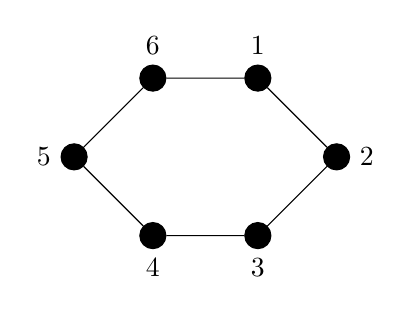
\begin{tikzpicture}
        \node[circle, draw, label={90:1}, fill=black] (1) at (2/3, 1) {};
        \node[circle, draw, label={0:2}, fill=black] (2) at (1+2/3, 0) {};
        \node[circle, draw, label={-90:3}, fill=black] (3) at (2/3, -1) {};
        \node[circle, draw, label={-90:4}, fill=black] (4) at (-2/3, -1) {};
        \node[circle, draw, label={180:5}, fill=black] (5) at (-1-2/3, 0) {};
        \node[circle, draw, label={90:6}, fill=black] (6) at (-2/3, 1) {};
        
        \draw (1) to (2)
            (2) to (3)
            (3) to (4)
            (4) to (5)
            (5) to (6)
            (6) to (1);
    \end{tikzpicture}
\end{figure}
\noindent We can view the symmetries of the hexagon as permutations inside $S_6$, through its action on the set of vertices. This corresponds to a group homomorphism from $D_6$ to $S_6$, where $r$ maps to $(123456)$ and $f$ maps to $(16)(25)(34)$. It turns out the homomorphism is completely determined by where we map $r$ and $f$, since every element in $D_6$ is of the form $r^a f^b$. Instead of considering the symmetries with respect to the vertices, we can consider the symmetries with respect to the diagonals of the hexagon.
\begin{figure}[H]
    \centering
    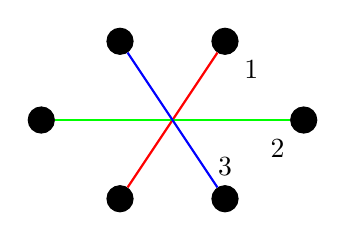
\begin{tikzpicture}
        \node[circle, draw, fill=black, label={-45:1}] (1) at (2/3, 1) {};
        \node[circle, draw, fill=black, label={-135:2}] (2) at (1+2/3, 0) {};
        \node[circle, draw, fill=black, label={90:3}] (3) at (2/3, -1) {};
        \node[circle, draw, fill=black] (4) at (-2/3, -1) {};
        \node[circle, draw, fill=black] (5) at (-1-2/3, 0) {};
        \node[circle, draw, fill=black] (6) at (-2/3, 1) {};
        
        \draw[thick, red] (1) to (4);
        \draw[thick, green] (2) to (5);
        \draw[thick, blue] (3) to (6);
    \end{tikzpicture}
\end{figure}
\noindent Now, the element $r$ corresponds to the permutation $(123)$, and $f$ corresponds to the permutation $(13)$. This too defines a group homomorphism, from $D_6$ to $S_3$. This map is not injective. In fact, the kernel of the homomorphism is $\{e, r^3\}$. Nonetheless, the map is surjective.

Now, we look at the first isomorphism theorem.
\begin{theorem}[First Isomorphism Theorem]
Let $G$ and $H$ be groups, and let $\varphi: G \to H$ be a group homomorphism. Then, $G/\ker (\varphi) \cong \operatorname{Im}(\varphi)$.
\end{theorem}
\begin{proof}
Let $K = \ker (\varphi)$. Define the map $\psi: G/\ker (\varphi) \to \operatorname{Im}(\varphi)$ by $\psi(gK) = \varphi(g)$. 
\begin{itemize}
    \item First, we show that $\psi$ is well-defined. Let $g_1K, g_2K \in G/\ker (\varphi)$. In that case, $g_1g_2^{-1} \in \ker (\varphi)$, and so
    \[\psi(g_1K)\psi(g_2k)^{-1} = \varphi(g_1)\varphi(g_2)^{-1} = \varphi(g_1 g_2^{-1}) = e_H.\]
    Therefore, $\psi(g_1K) = \psi(g_2K)$. So, $\psi$ is well-defined.
    \item Next, we show that $\psi$ is a homomorphism. Let $g_1K, g_2K \in G/\ker (\varphi)$. In that case,
    \[\psi(g_1K)\psi(g_2K) = \varphi(g_1) \varphi(g_2) = \varphi(g_1g_2) = \psi(g_1g_2).\]
    So, $\psi$ is a homomorphism.
    \item Now, we show that $\psi$ is injective. Assume that $gK \in \ker (\psi)$. Therefore, 
    \[\varphi(g) = \psi(gK) = e_H.\]
    So, $g \in \ker (\varphi)$. This implies that $gK = K$. Therefore, $\ker \psi = \{K\}$. So, $\psi$ is injective.
    \item Finally, we show that $\psi$ is surjective. Let $h \in \operatorname{Im}(\varphi)$. By definition, there exists a $g \in G$ such that $\varphi(g) = h$. In that case,
    \[\psi(gH) = \varphi(g) = h.\]
    So, $\psi$ is surjective.
\end{itemize}
Therefore, $\psi$ is an isomorphism. This implies that $G/\ker (\varphi) \cong \operatorname{Im}(\varphi)$.
\end{proof}
\noindent We can think of the First Isomorphism Theorem intuitively. Let $G$ and $H$ be groups and let $\varphi: G \to H$ be a group homomorphism. If we limit the map to $\operatorname{Im}(\varphi)$, then the map will be surjective. Now, consider the equivalence relation $\sim$ on $G$ given by
\[g_1 \sim g_2 \iff \varphi(g_1) = \varphi(g_2).\]
If we quotient $G$ by this relation, then the map will be injective- if two values $g_1, g_2 \in G$ map to the same value, then the two values will lie in the same equivalence class under $\sim$. Now, for $g_1, g_2 \in G$, $\varphi(g_1) = \varphi(g_2)$ if and only if $\varphi(g_1g_2^{-1}) = e_H$, and $\varphi(g_1g_2^{-1}) = e_H$ if and only if $g_1g_2^{-1} \in \ker (\varphi)$. Moreover, $g_1 g_2^{-1} \in \ker (\varphi)$ if and only if $g_1 \cdot \ker (\varphi) = g_2 \cdot \ker (\varphi)$. This is the property we used in the theorem above- quotienting by $\sim$ is the same as quotienting by the kernel. Alternatively, we know that the function is injective if and only if the kernel is trivial. So, if we quotient by the kernel, then the kernel will be trivial under the quotient. This ensures that we have a bijection from $G/\ker (\varphi) \cong \operatorname{Im}(\varphi)$.

We will now consider some applications of the First Isomorphism Theorem. First, consider the group $D_6$ and consider the symmetries in $D_6$ with respect to the diagonals of the hexagon. We saw this example above- the picture is given below as well.
\begin{figure}[H]
    \centering
    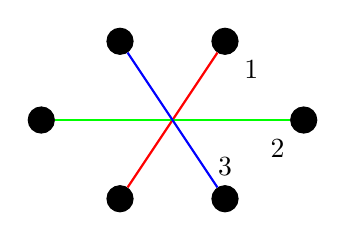
\begin{tikzpicture}
        \node[circle, draw, fill=black, label={-45:1}] (1) at (2/3, 1) {};
        \node[circle, draw, fill=black, label={-135:2}] (2) at (1+2/3, 0) {};
        \node[circle, draw, fill=black, label={90:3}] (3) at (2/3, -1) {};
        \node[circle, draw, fill=black] (4) at (-2/3, -1) {};
        \node[circle, draw, fill=black] (5) at (-1-2/3, 0) {};
        \node[circle, draw, fill=black] (6) at (-2/3, 1) {};
        
        \draw[thick, red] (1) to (4);
        \draw[thick, green] (2) to (5);
        \draw[thick, blue] (3) to (6);
    \end{tikzpicture}
\end{figure}
\noindent It defines a homomorphism from $D_6$ to $S_3$. We saw that the homomorphism is surjective, with kernel $H = \{e, r^3\}$. Therefore, the first isomorphism theorem tells us that $D_6/H \cong S_3$. Next, consider the group of non-zero complex numbers $\mathbb{C}^\times$ under multiplication. We know that the function $f: \mathbb{R} \to \mathbb{C}^{\times}$ given by $f(x) = e^{2\pi ix}$ is a group homomorphism. That is, for $x, y \in \mathbb{R}$,
\[f(x + y) = e^{2\pi i(x + y)} = e^{2\pi ix} \cdot e^{2\pi iy}.\]
Its image is the unit circle in the complex plane:
\[S^1 = \{z \in \mathbb{C} \mid |z| = 1\}.\]
Its kernel is $\mathbb{Z}$- if $x \in \mathbb{Z}$, then $e^{2\pi ix} = 1$. Therefore, the First Isomorphism Theorem tells us that $\mathbb{R}/\mathbb{Z} \cong S^1$. In $\mathbb{R}/\mathbb{Z}$, the different cosets are composed of different decimal expansions- this tells us that there is a bijection from the decimal expansions to the unit circle. Now, consider the group homomorphism from $\mathbb{C}^\times$ to $\mathbb{R}_{> 0}$ given by $z \mapsto |z|$. We know that for all $z_1, z_2 \in \mathbb{C}^\times$, $|z_1 z_2| = |z_1| |z_2|$, so this function defines a group homomorphism. This map is surjective, since for $x \in \mathbb{R}_{> 0}$, $|x| = x$. The kernel of the homomorphism is the elements with modulus 1, i.e. $S^1$. Here, the first isomorphism theorem tells us that $\mathbb{C}^\times/S^1 \cong \mathbb{R}_{> 0}$. In fact, we have $\mathbb{C}^\times \cong S^1 \times \mathbb{R}_{> 0}$. This is because $S^1 \cap \mathbb{R}_{> 0} = \{1\}$ and for every $z \in \mathbb{C}$, we can write $z = |z| \cdot e^{i \omega}$, for some $\omega \in [0, 2\pi)$.\sidefootnote{These two properties imply that $C^\times \cong S^1 \times \mathbb{R}_{> 0}$- we shall prove this later!}

Now, we shall use the first isomorphism theorem to classify the group homomorphisms from the cyclic group of order 4, $\mathbb{Z}/4 \mathbb{Z}$, to the cyclic group of order 10, $\mathbb{Z}/10 \mathbb{Z}$.
\begin{example}
There are 2 group homomorphisms from $\mathbb{Z}/4 \mathbb{Z}$ to $\mathbb{Z}/10 \mathbb{Z}$.
\end{example}
\begin{proof}
Let $\varphi: \mathbb{Z}/4 \mathbb{Z} \to \mathbb{Z}/10 \mathbb{Z}$ be a group homomorphism. We consider all the possible kernels:
\begin{itemize}
    \item We can have $\ker (\varphi) = \{0 + 4\mathbb{Z}\}$. In that case, the First Isomorphism Theorem tells us that $G/\ker (\varphi) \cong \operatorname{Im}(\varphi)$. Since $\ker (\varphi) = \{0 + 4\mathbb{Z}\}$, we find that $G/\ker (\varphi) \cong G$, and $\operatorname{Im}(\varphi) \leqslant H$. So, we require $\operatorname{Im}(\varphi)$ to be a cyclic subgroup of $\mathbb{Z}/10 \mathbb{Z}$, of order 4. However, Lagrange's Theorem tells us that a subgroup of $\mathbb{Z}/10 \mathbb{Z}$ has order either 1, 2, 5 or 10. Therefore, we cannot have $\ker (\varphi) = \{0 + 4\mathbb{Z}\}$.
    
    \item We can have $\ker (\varphi) = \{0 + 4\mathbb{Z}, 2 + 4\mathbb{Z}\}$. In that case, the First Isomorphism Theorem tells us that $G/\ker (\varphi) \cong \operatorname{Im}(\varphi)$. Since $|\ker (\varphi)| = 2$, we find that 
    \[|\operatorname{Im}(\varphi)| = \frac{|G|}{|\ker (\varphi)|} = \frac{4}{2} = 2.\]
    There is precisely one subgroup of $\mathbb{Z}/10 \mathbb{Z}$ with order $2$- $\{0 + 10\mathbb{Z}, 5 + 10\mathbb{Z}\}$, so there is precisely one isomorphism\sidefootnote{This is not true for every possible order! For example, there are 2 homomorphisms from $\mathbb{Z}/4\mathbb{Z}$ to $\mathbb{Z}/4\mathbb{Z}$ with $\ker (\varphi) = \{0 + 4\mathbb{Z}\}$ and $\operatorname{Im}(\varphi) = \mathbb{Z}/4\mathbb{Z}$.}. Therefore, if $\ker (\varphi) = \{0 + 4\mathbb{Z}, 2 + 4\mathbb{Z}\}$, then $\varphi(1 + 4\mathbb{Z}) = 5 + 10\mathbb{Z}$.
    
    \item We can also have $\ker (\varphi) = \mathbb{Z}/4 \mathbb{Z}$. In that case, for all $n + 4\mathbb{Z} \in \mathbb{Z}/4 \mathbb{Z}$, $\varphi(n + 4\mathbb{Z}) = 10 \mathbb{Z}$. This gives us precisely one homomorphism- the trivial homomorphism.
\end{itemize}
Therefore, there are 2 homomorphisms from $\mathbb{Z}/4 \mathbb{Z}$ to $\mathbb{Z}/10 \mathbb{Z}$.
\end{proof}
We can think of normal subgroups as precisely those that are kernels of some homomorphism.
\begin{proposition}
Let $G$ be a group and let $H \leqslant G$. Then, $H$ is a normal subgroup if and only if there exists a group $K$ and a group homomorphism $\varphi: G \to K$ such that $\ker (\varphi) = H$.
\end{proposition}
\begin{proof}
We know that the kernel of a group homomorphism is a normal subgroup. Moreover, the quotient map $\varphi: G \to G/H$ given by $\varphi(g) = gH$ has kernel:
\begin{align*}
    \ker (\varphi) &= \{g \in G \mid \varphi(g) = H\} \\
    &= \{g \in G \mid gH = H\} \\
    &= \{g \in G \mid g \in H\} = H.
\end{align*}
\end{proof}
We shall now use the First Isomorphism Theorem to prove the Second Isomorphism Theorem.
% TODO: Show HN is subgroup + Image is HN/N better!
\begin{theorem}[Second Isomorphism Theorem]
Let $G$ be a group, $H \leqslant G$ and $N \vartriangleleft G$. Then,
\begin{itemize}
    \item the set 
    \[HN = \{hn \mid h \in H, n \in N\}\]
    is a subgroup of $G$;
    \item the intersection $H \cap N$ is a normal subgroup of $H$; and
    \item there is an isomorphism $H/(H \cap N) \cong HN/N$.
\end{itemize}
\end{theorem}
\begin{proof}
Define the map $\varphi: H \to G/N$ by $\varphi(h) = hN$. 
\begin{itemize}
    \item For $h_1, h_2 \in H$, we have
    \[\varphi(h_1h_2) = (h_1h_2)N = h_1N h_2N = \varphi(h_1) \varphi(h_2),\]
    so $\varphi$ is a group homomorphism.
    
    \item Moreover, the kernel of the map is given by
    \begin{align*}
        \ker (\varphi) &= \{h \in H \mid \varphi(h) = N\} \\
        &= \{h \in H \mid hN = N\} \\
        &= \{h \in H \mid h \in N\} = H \cap N.
    \end{align*}
    This implies that $H \cap N$ is a normal subgroup of $H$. 
    
    \item Now, we show that the image $\operatorname{Im}(\varphi) = HN/N$. First, assume that $h \in H$. Since $e \in N$, we find that $h \in HN$. In that case, 
    \[\varphi(h) = hN \in HN/N.\]
    Now, let $hn \in HN$. In that case,
    \[\varphi(h) = hN = hnN.\]
    This implies that $\operatorname{Im}(\varphi) = HN/N$. We know that $HN/N \leqslant G/N$, so $HN \leqslant G$.
\end{itemize}
Therefore, the First Isomorphism Theorem tells us that
\[H/(H \cap N) = H/\ker (\varphi) \cong \operatorname{Im}(\varphi) = HN/N.\]
\end{proof}
\noindent We can think of it in a different way. Let $G$ be a group, $H \leqslant G$ and $N \vartriangleleft G$. We know that for the map $\varphi: G \to G/N$, the First Isomorphism Theorem tells us that $G/\ker \varphi \cong G/N$. Now, consider what happens when we replace $G$ with the subgroup $H$. Consider the restricted homomorphism $\varphi|_H: H \to G/N$. This is precisely the map we used above to prove the Second Isomorphism Theorem. Therefore, the Second Isomorphism Theorem is the application of the First Isomorphism Theorem to a subgroup of $G$.

We now look at an example of the Second Isomorphism Theorem. Let $\operatorname{GL}_2(\mathbb{R})$ be the multiplicative group of all $2 \times 2$ invertible matrices over $\mathbb{R}$. Let $\operatorname{SL}_2(\mathbb{R}) \leqslant \operatorname{GL}_2(\mathbb{R})$ be the subgroup consisting of matrices with determinant 1. This is a normal subgroup since $\operatorname{SL}_2(\mathbb{R})$ is the kernel of the determinant homomorphism $\det: \operatorname{GL}_2(\mathbb{R}) \to \mathbb{R}^{\times}$. Moreover, we can apply the First Isomorphism Theorem to this homomorphism to find that $\operatorname{GL}_2(\mathbb{R})/\operatorname{SL}_2(\mathbb{R}) \cong \mathbb{R}^{\times}$. Now, consider the subgroup
\[Z = \left\{\begin{bmatrix}
a & 0 \\
0 & a
\end{bmatrix} \mid a \in \mathbb{R}^{\times}\right\}\]
of $\operatorname{GL}_2(\mathbb{R})$. For a matrix $A \in Z$ with
\[A = \begin{bmatrix}
a & 0 \\
0 & a
\end{bmatrix},\]
we have $\det (A) = a^2$. Therefore, the intersection $Z \cap \operatorname{GL}_2(\mathbb{R}) = \{\mathbb{I}_2, - \mathbb{I}_2\}$. Moreover,
\[Z \cdot \operatorname{SL}_2(\mathbb{R}) = \{A \in \operatorname{GL}_2(\mathbb{R}) \mid \det (A) > 0\}.\]
We prove this now. So, let $A \in Z$ and $B \in \operatorname{SL}_2(\mathbb{R})$, with
\[A = \begin{bmatrix}
a & 0 \\
0 & a
\end{bmatrix}.\]
Then,
\[\det(AB) = \det(A) \det(B) = a^2 \cdot \det(B) = a^2 > 0.\]
Now, let $A \in \operatorname{GL}_2(\mathbb{R})$ with $\det(A) > 0$. Set $\det(A) = a$. Define the matrix
\[B = \begin{bmatrix}
\sqrt{a} & 0 \\
0 & \sqrt{a}
\end{bmatrix} \in Z.\]
Let $C = AB^{-1}$. We have
\[\det(C) = \det(A) \det(B^{-1}) = a \cdot \frac{1}{a} = 1,\]
so $C \in \operatorname{SL}_2(\mathbb{R})$. Moreover, $A = BC \in Z \cdot \operatorname{SL}_2(\mathbb{R})$. This proves the set equality
\[Z \cdot \operatorname{SL}_2(\mathbb{R}) = \{A \in \operatorname{GL}_2(\mathbb{R}) \mid \det (A) > 0\} = \operatorname{GL}_2^+ (\mathbb{R}).\]
In that case, the Second Isomorphism Theorem tells us that
\[Z/\{\mathbb{I}_2, -\mathbb{I}_2\} \cong \operatorname{GL}_2^+(\mathbb{R})/ \operatorname{SL}_2(\mathbb{R}).\]
Now, we consider applying the First Isomorphism Theorem directly to the determinant map $\det: Z \to \mathbb{R}^\times$. We know that for all $A \in Z$, $\det(A) > 0$. Moreover, $\ker (\det) = \{\mathbb{I}_2, -\mathbb{I}_2\}$. So, $Z/\{\mathbb{I}_2, -\mathbb{I}_2\} \cong \mathbb{R}_{> 0}$ by the First Isomorphism Theorem. Also, we find that $\operatorname{GL}_2^+(\mathbb{R})/\operatorname{SL}_2(\mathbb{R}) \cong \mathbb{R}_{> 0}$ using the determinant map and the first isomorphism theorem again.

Next, we look at an application of the Second Isomorphism Theorem. We start by defining metabelian groups.
\begin{definition}
Let $G$ be a group. Then $G$ is \emph{metabelian} if there exists a normal subgroup $N$ of $G$ such that both $G/N$ and $N$ are abelian.
\end{definition}
\noindent Using the Second Isomorphism Theorem, we can prove that any subgroup of a metabelian group is metabelian.
\begin{proposition}
Let $G$ be a metabelian group, and let $H \leqslant G$. Then, $H$ is metabelian.
\end{proposition}
\begin{proof}
Since $G$ is a metabelian group, there exists a normal subgroup $N$ such that $N$ and $G/N$ is abelian. In that case, the Second Isomorphism Theorem tells us that $H \cap N$ is normal in $H$, and
\[H/(H \cap N) \cong HN/N.\]
We have $HN/N \leqslant G/N$, so $HN/N$ is abelian. Therefore, $H/(H \cap N)$ is abelian. Moreover, $H \cap N$ is a subgroup of the abelian group $N$, so $H \cap N$ too is abelian. Therefore, $H$ is metabelian.
\end{proof}

Next, we look at the Third Isomorphism Theorem.
\begin{theorem}[Third Isomorphism Theorem]
Let $G$ be a group, and let $N \vartriangleleft H$, and let $\pi: G \to G/N$ be the quotient map. Then,
\begin{itemize}
    \item for a subgroup $U \leqslant G/N$, the preimage
    \[\pi^{-1}(U) = \{g \in G \mid \pi(g) \in U\}\]
    is a subgroup of $G$ containing $N$;
    \item if $U$ is a subgroup of $G/N$, then $U$ is normal in $G/N$ if and only if $\pi^{-1}(U)$ is normal in $G$; 
    \item the function $U \mapsto \pi^{-1}(U)$ defines a bijection between the set of subgroups of $G/N$ and the subgroups of $G$ containing $N$;
    \item if $K$ is a normal subgroup of $G$ containing $N$, then $\pi$ defines an isomorphism
    \[G/K \cong (G/N)/(K/N).\]
\end{itemize}
\end{theorem}
\begin{proof}
\hspace*{0pt}
\begin{itemize}
    \item Let $U \leqslant G/N$. Define
    \[H = \pi^{-1}(U) = \{g \in G \mid \pi(g) \in U\}.\]
    We have $N \in G/N$, so $N \subseteq H$. Let $g_1, g_2 \in H$. In that case, we know that $\pi(g_1), \pi(g_2) \in U$. Since $U$ is a subgroup of $G/N$, we know that
    \[\pi(g_1 g_2^{-1}) = \pi(g_1) \pi(g_2)^{-1} \in U.\]
    So, $g_1 g_2^{-1} \in H$. Since $e_H \in U$, we have $e_G \in H$. Therefore, the subgroup test tells us that $H$ is a subgroup of $G$.
    
    \item \begin{itemize}
        \item First, assume that $U \vartriangleleft G/N$. We know that $\pi^{-1}(U)$ is a subgroup of $G$. So, let $g \in G$ and $h \in \pi^{-1}(U)$. Since $U$ is normal in $G/N$,
        \[\varphi(ghg^{-1}) = \varphi(g) \varphi(h) \varphi(g)^{-1} \in U.\]
        Therefore, $ghg^{-1} \in \pi^{-1}(U)$. This implies that $\pi^{-1}(U)$ is a normal subgroup of $G$.
        
        \item Now, assume that $U \leqslant G/N$ such that $\pi^{-1}(U)$ is normal in $G/H$. Let $gH = \pi(g) \in G/H$ and $xH = \pi(x) \in U$. Since $g \in G$ and $x \in \pi^{-1}(U)$, we find that $gxg^{-1} \in \pi^{-1}(U)$. In that case,
        \[\pi(g) \pi(x) \pi(g)^{-1} = \pi(g) \pi(x) \pi(g^{-1}) = \pi(gxg^{-1}) \in U.\]
        Therefore, $U$ is normal in $G/N$.
    \end{itemize}
    
    \item The inverse function of $U \mapsto \pi^{-1}(U)$ is $H \mapsto \pi(H)$. So, the function is bijective since $H$ is a subgroup that contains $N$.
    
    \item We show that the function $\varphi: G/K \to (G/N)/(K/N)$ given by $\varphi(gK) = gN(K/N)$ is an isomorphism.
    \begin{itemize}
        \item First, we show that $\varphi$ is well-defined. So, let $g_1K, g_2K \in G/K$ such that $g_1K = g_2K$. In that case, $g_2 g_1^{-1} \in K$. So, $g_2 g_1^{-1}N \in K/N$. This implies that 
        \[\varphi(g_1) = g_1N(K/N) = g_2N(K/N) = \varphi(g_2).\]
        Therefore, $\varphi$ is well-defined.
        
        \item Next, we show that $\varphi$ is a homomorphism. So, let $g_1K, g_2K \in G/K$. Then,
        \begin{align*}
            \varphi(g_1K \cdot g_2K) &= \varphi(g_1g_2K) = g_1g_2N (K/N) \\
            &= (g_1N (K/N)) (g_2N (K/N)).
        \end{align*}
        Therefore, $\varphi$ is a homomorphism.
        
        \item Now, we show that $\varphi$ is injective. So, let $g_1K, g_2K \in G/K$ such that $\varphi(g_1K) = \varphi(g_2K)$. In that case, $g_1N (K/N) = g_2N (K/N)$. This implies that 
        \[(g_2N)^{-1}(g_1N) = g_2^{-1}g_1N \in K/N.\]
        So, there exists a $k \in K$ such that $g_2^{-1}g_1N = kN$. In that case, 
        \[(k^{-1})g_2^{-1}g_1 \in N \leqslant K.\]
        By closure, this implies that $g_2^{-1}g_1 \in K$. So, $g_1K = g_2K$. Therefore, $\varphi$ is injective.
        
        \item Finally, we show that $\varphi$ is surjective. So, let \\ $gN(K/N) \in (G/N)/(K/N)$. We have $\varphi(gK) = gN(K/N)$. Therefore, $\varphi$ is surjective.
    \end{itemize}
    This implies that $\varphi$ is an isomorphism. So, $G/K \cong (G/N)/(K/N)$.
\end{itemize}
\end{proof}
\noindent We can think of the Third Isomorphism Theorem intuitively. Essentially, it states that for a group $G$, a normal subgroup $K$, and a homomorphism $\varphi$ from $G$ such that $\ker (\varphi) \leqslant K$, then
\[G/K \cong \varphi(G)/\varphi(K).\]

Next, we look at some examples of the Third Isomorphism Theorem. Let $G = \operatorname{GL}_2(\mathbb{R})$, and let 
\[K = \operatorname{GL}_2^+(\mathbb{R}) = \{X \in \operatorname{GL}_2(\mathbb{R}) \mid \det(X) > 0\}.\]
The subgroup $K$ of $G$ is normal- for matrices, $A \in \operatorname{GL}_2(\mathbb{R}), B \in \operatorname{GL}_2^+(\mathbb{R})$,
\[\det(ABA^{-1}) = \det(A) \det(B) \det(A)^{-1} = \det(B) > 0.\]
We want to understand the structure of the quotient group $G/K$ using the Third Isomorphism Theorem. So, let $N = \operatorname{SL}_2(\mathbb{R})$. We know that $N$ is a normal subgroup of $G$- it is the kernel of the determinant map. Moreover, $N \leqslant K$. We have two surjective homomorphisms: $\det: \operatorname{GL}_2(\mathbb{R}) \to \mathbb{R}^\times$ and $\det: \operatorname{GL}_2^+(\mathbb{R}) \to \mathbb{R}_{> 0}$. So, the Third Isomorphism Theorem tells us that
\[G/K \cong \det(G)/\det(K) = \mathbb{R}^\times/\mathbb{R}_{> 0}.\]
Moreover, these quotient groups are isomorphic to the cyclic group of order 2.

\newpage

\section{Group Actions}
\subsection{Definition of Group Actions}
We will now review group actions.
\begin{definition}
Let $G$ be a group and $X$ be a set. A \emph{left action} of $G$ on $X$ is a function $\cdot: G \times X \to X$ such that
\begin{itemize}
    \item $e \cdot x = x$ for all $x \in X$; and
    \item $g_1 \cdot (g_2 \cdot x) = (g_1 g_2) \cdot x$ for all $g_1, g_2 \in G$ and $x \in X$.
\end{itemize}
If $\cdot$ defines a group action, then we say that $X$ is a \emph{$G$-set}.
\end{definition}
\noindent A right action is defined analogously. We will typically assume the action to a left action, unless specified.

A group action from a group $G$ to a set $X$ can be thought of as a set of functions from $X$ to itself. That is, for every $g \in G$, we have a function from $X$ to itself, given by $g \cdot x$. It turns out that this function is bijective.
\begin{proposition}
Let $G$ be a group and let $X$ be a $G$-set, and let $g \in G$. Define the function $\sigma_g: X \to X$ defined by $\sigma_g(x) = g \cdot x$ is bijective.
\end{proposition}
\begin{proof}
\hspace*{0pt}
\begin{itemize}
    \item We first show that $\sigma_g$ is injective. Now, let $x_1, x_2 \in X$ such that $\sigma_g(x_1) = \sigma_g(x_2)$. Therefore, $g \cdot x_1 = g \cdot x_2$. In that case,
    \[x_1 = (g^{-1}g) \cdot x_1 = g^{-1} \cdot (g \cdot x_1) = g^{-1} \cdot (g \cdot x_2) = (g^{-1}g) \cdot x_2 = x_2.\]
    Therefore, $\sigma_g$ is injective.
    \item We now show that $\sigma_g$ is surjective. So, let $x \in X$. We find that
    \[\sigma_g(g^{-1} \cdot x) = g \cdot (g^{-1} \cdot x) = (gg^{-1}) \cdot x = e \cdot x = x.\]
    Therefore, $\sigma_g$ is surjective.
\end{itemize}
So, $\sigma_g$ is bijective.
\end{proof}
\noindent Moreover, this is a group homomorphism from the group to the symmetries of $X$, defined by the group action.
\begin{proposition}
Let $G$ be a group and let $X$ be a $G$-set. For $g \in G$, define the function $\sigma_g: X \to X$ by $\sigma_g(x) = g \cdot x$. Then, the map $\varphi: G \to S_X$ defined by $\varphi(g) = \sigma_g$ is a group homomorphism.
\end{proposition}
\begin{proof}
We know that $\sigma_g$ is bijective for all $g \in G$. Therefore, $\sigma_g \in S_X$, the map is well-defined. Now, for $g_1, g_2 \in G$ and $x \in X$
\begin{align*}
    (\varphi(g_2) \circ \varphi(g_2))(x) &= (\sigma_{g_2} \circ \sigma_{g_1}) \cdot x \\
    &= \sigma_{g_2}(\sigma_{g_1}(x)) \\
    &= \sigma_{g_2} (g_1 \cdot x) \\
    &= g_2 \cdot (g_1 \cdot x) \\
    &= (g_2g_1) \cdot x \\
    &= \sigma_{g_2g_1}(x) = \varphi(g_2g_1)(x).
\end{align*}
Therefore, $\varphi(g_2) \circ \varphi(g_1) = \varphi(g_1 g_2)$. This implies that $\varphi$ is a group homomorphism.
\end{proof}

We now look at some examples of group actions. Let $n \in \mathbb{Z}_{\geq 1}$, $G = S_n$, and
\[X = \{1, 2, \dots, n\}.\]
Then, the group $G$ acts naturally on $X$ by permutation. For instance, we have $(123)(1) = 2$ in $S_3$. Now, let $n \in \mathbb{Z}_{\geq 3}$. Then, the dihedral group $D_n$ acts on the set of vertices (and the edges) of a regular $n$-gon. Now, let $G$ be the group of rotations of a cube. Then, $G$ acts on the set of diagonals of the cube. The picture below shows the 4 long diagonals.
% TODO: Draw => Label each vertex of the cube
Each rotation of the cube permutes the diagonals. This defines a group homomorphism from $G$ to $S_4$. In fact, this map is an isomorphism.

Now, we define transitive group actions.
\begin{definition}
Let $G$ be a group and let $X$ be a $G$-set. Then, the action is called \emph{transitive} if for all $x, y \in X$, there exists a $g \in G$ such that $g \cdot x = y$.
\end{definition}
\noindent So, an action is transitive if we can go between any two elements in $X$. We now look at an example of transitive group actions. Let $G$ be a group and $H \leq G$. Then, the group acts on the set of left cosets by the map $g \cdot xH = gxH$. This action is transitive since for all $xH, yH \in G/H$, $(yx^{-1}) \cdot xH = yH$.

Like groups, $G$-sets can also be isomorphic.
\begin{definition}
Let $G$ be a group, and let $X$ and $Y$ be $G$-sets. an \emph{isomorphism} from $X$ to $Y$ is a bijection $\phi: X \to Y$ such that for all $x \in X$ and $g \in G$, $\phi(g \cdot x) = g \cdot \phi(x)$.
\end{definition}
\noindent It turns out that only conjugate subgroups are isomorphic as $G$-sets with respect to the coset group action.
\begin{proposition}
Let $G$ be a group and let $H$ and $K$ be subgroups of $G$. Then, the $G$-sets $G/H$ and $G/K$ are isomorphic if and only if there exists a $g \in G$ such that $H = gKg^{-1}$.
\end{proposition}
\begin{proof}
\hspace*{0pt}
\begin{itemize}
    \item First, assume that there exists a $g \in G$ such that $H = gKg^{-1}$. Define the function $\phi: G/H \to G/K$ by $\phi(xH) = xgK$.\sidefootnote{Note that the map $xH \mapsto xK$ is not well-defined! To construct this map, we consider where the identity coset $H$ gets mapped to. Let $\phi(H) = aK$. In that case, for all $h \in H$, $aK = \varphi(H) = \varphi(hH)  = h \cdot \varphi(H) = h \cdot aK = haK$. So, we need $a^{-1}ha \in K$. Since $K = g^{-1}Hg$, we choose $a = g$. In that case, for $x \in G$, we have $\phi(xH) = \phi(x \cdot H) = x \cdot \phi(H) = xgK$.} We show that $\phi$ is a well-defined isomorphism:
    \begin{itemize}
        \item So, let $x_1H = x_2H$. In that case, $x_2^{-1}x_1 \in H$. Since $H = gKg^{-1}$, we find that $x_2^{-1}x_1 = gkg^{-1}$ for some $k \in K$. In that case, 
        \[(x_2g)^{-1} (x_1g) = g^{-1}x_2^{-1} x_1g = k \in K.\]
        This implies that $\phi(x_1g) = x_1gK = x_2gK = \phi(x_2g)$. So, $\phi$ is well-defined.
        
        \item Now, let $x_1H, x_2H \in G/H$ such that $\phi(x_1H) = \phi(x_2H)$. In that case, $x_1gK = x_2gK$. This implies that 
        \[(x_2g)^{-1}(x_1g) = g^{-1}x_2^{-1}x_1g \in K.\]
        Since $g^{-1}Hg = K$, we find that $x_2^{-1}x_1 \in H$. Therefore, $x_1H = x_2H$. So, $\phi$ is injective.
        
        \item Next, let $yK \in G/K$. In that case,
        \[\phi(yg^{-1} H) = yg^{-1} (gK) = yK.\]
        So, $\phi$ is surjective.
        
        \item Finally, let $xH \in G/H$ and $y \in G$. Then,
        \[\phi(y \cdot xH) = \phi(yxH) = yxgK = y \cdot xgK = y \cdot \phi(xH).\]
    \end{itemize}
    This implies that $\phi$ is an isomorphism.
    
    \item Now, assume that $G/H$ and $G/K$ are isomorphic. In that case, there exists a bijective function $\phi: G/H \to G/K$ such that for all $y \in G$ and $xH \in G/H$, $\phi(y \cdot xH) = y \cdot \phi(xH)$. In that case, fix a $g \in G$ such that $g \in \phi(H)$, i.e. $\phi(H) = gK$. We show that $H = gKg^{-1}$.
    \begin{itemize}
        \item Assume that $h \in H$. In that case,
        \[gK = \phi(H) = \phi(hH) = h \cdot \phi(H) = h \cdot gK = hgK.\]
        This implies that $g^{-1}hg \in K$. So, let $k \in K$ such that $g^{-1}hg = k$. Therefore, $h = gkg^{-1} \in gKg^{-1}$.
        
        \item Assume that $x \in gKg^{-1}$. In that case, there exists a $k_1 \in K$ such that $x = gk_1 g^{-1}$. This implies that
        \begin{align*}
            \phi(x \cdot H) &= x \cdot \phi(H) \\
            &= x \cdot gK \\
            &= gk_1g^{-1} \cdot gK \\
            &= gk_1K \\
            &= gK \\
            &= \phi(H).
        \end{align*}
        Since $\phi$ is injective, we find that $x \cdot H = H$. Therefore, $x \in H$.
    \end{itemize}
    So, $H = gKg^{-1}$.
\end{itemize}
This implies that $G/H$ and $G/K$ are isomorphic if and only if there exists a $g \in G$ such that $H = gKg^{-1}$.
\end{proof}

\subsection{Orbit-Stabiliser Theorem}
Now, we will look at the Orbit-Stabiliser Theorem. We start by defining orbits and stabilisers.
\begin{definition}
Let $G$ be a group, let $X$ be a $G$-set, and let $x \in X$. The \emph{orbit} of $x$ is the set
\[\operatorname{Orb}_G(x) = \{g \cdot x \mid g \in G\}.\]
The \emph{stabiliser} of $x$ is the set
\[\operatorname{Stab}_G(x) = \{g \in G \mid g \cdot x = x\}.\]
\end{definition}
\noindent Note that the orbit is a subset of $X$, while the stabiliser is a subset of $G$. In fact, the stabiliser turns out to be a subgroup.
\begin{proposition}
Let $G$ be a group, let $X$ be a $G$-set, and let $x \in X$. Then, the stabiliser $\operatorname{Stab}_G(x)$ is a subgroup of $G$.
\end{proposition}
\begin{proof}
Let $g_1, g_2 \in \operatorname{Stab}_G(x)$. In that case, $g_1 \cdot x = x$ and $g_2 \cdot x = x$. Therefore,
\[g_2^{-1} \cdot x = g_2^{-1} \cdot (g_2 \cdot x) = (g_2^{-1}g_2) \cdot x = e \cdot x = x.\]
In that case,
\[(g_1 g_2^{-1}) \cdot x = g_1 \cdot (g_2^{-1} \cdot x) = g_1 \cdot x = x.\]
Since $e \in \operatorname{Stab}_G(x)$, we find that $\operatorname{Stab}_G(x)$ is a subgroup, using the subgroup test.
\end{proof}
\noindent We now show that the orbits form an equivalence relation.
\begin{proposition}
Let $G$ be a group, and let $X$ be a $G$-set. Define the relation $\sim$ on $X$ by
\[x_1 \sim x_2 \iff x_2 \in \operatorname{Orb}_G(x_1).\]
Then, $\sim$ is an equivalence relation.
\end{proposition}
\begin{proof}
\hspace*{0pt}
\begin{itemize}
    \item Let $x \in X$. Since $e \cdot x = x$, $x \in \operatorname{Orb}_G(x)$. So, $x \sim x$.
    
    \item Let $x, y \in X$ such that $x \sim y$. In that case, $y \in \operatorname{Orb}_G(x)$. This implies that there exists a $g \in G$ such that $y = g \cdot x$. In that case,
    \[g^{-1} \cdot y = g^{-1} \cdot (g \cdot x) = (g^{-1} g) \cdot x = e \cdot x = x.\]
    Therefore, $x \in \operatorname{Orb}_G(y)$. So, $y \sim x$.
    
    \item Let $x, y, z \in X$ such that $x \sim y$ and $y \sim z$. In that case, $y \in \operatorname{Orb}_G(x)$ and $z \in \operatorname{Orb}_G(y)$. Therefore, there exist $g_1, g_2 \in G$ such that $y = g_1 \cdot x$ and $z = g_2 \cdot y$. This implies that
    \[z = g_2 \cdot y = g_2 \cdot (g_1 \cdot x) = g_2g_1 \cdot x.\]
    So, $z \in \operatorname{Orb}_G(x)$. So, $x \sim z$.
\end{itemize}
This implies that $\sim$ is an equivalence relation.
\end{proof}
\noindent Clearly, the partitions induced by this relation are the orbits. Next, we show that the stabiliser of two elements in the same orbit are conjugate.
\begin{proposition}
Let $G$ be a group, and let $X$ be a $G$-set. Then, for $x, y \in X$, there exists a $g \in G$ such that $\operatorname{Stab}_G(x) = g \operatorname{Stab}_G(y) g^{-1}$ if and only if $\operatorname{Orb}_G(x) = \operatorname{Orb}_G(y)$.
\end{proposition}
\begin{proof}
\hspace*{0pt}
\begin{itemize}
    \item Assume that $\operatorname{Orb}_G(x) = \operatorname{Orb}_G(y)$. In that case, there exists a $g \in G$ such that $y = g \cdot x$. We show that $\operatorname{Stab}_G(x) = g \operatorname{Stab}_G(y) g^{-1}$. So, let $h \in X$. We know that $h \in \operatorname{Stab}_G(x)$ if and only if
    \begin{align*}
        (ghg^{-1}) \cdot y &= g \cdot (h \cdot (g^{-1} \cdot y)) \\
        &= g \cdot (h \cdot x) \\
        &= g \cdot x = y.
    \end{align*}
    Therefore, $h \in \operatorname{Stab}_G(x)$ if and only if $ghg^{-1} \in \operatorname{Stab}_G(y)$. This implies that $\operatorname{Stab}_G(y) = g^{-1} \operatorname{Stab}_G(x) g$. So, $\operatorname{Stab}_G(x) = g \operatorname{Stab}_G(y) g^{-1}$.
    
    \item Now, assume that there exists a $g \in G$ such that 
    \[\operatorname{Stab}_G(x) = g \operatorname{Stab}_G(y) g^{-1}.\]
    So, let $h_1 \in \operatorname{Stab}_G(x)$. By definition, we have $h_1 \cdot x = x$. We also know that there exists an $h_2 \in \operatorname{Stab}_G(y)$ such that $h_1 = gh_2g^{-1}$.
    % TODO: Prove (DON'T GOOGLE!)
\end{itemize}
\end{proof}
% TODO: Lc 15 => What is conjugacy class? Doesn't look like the normal definition! Also, the stabiliser for a transitive G-set is trivial?
\noindent Next, we show that every transitive $G$-set is isomorphic to left cosets of some subgroup of $G$.
\begin{proposition}
Let $G$ be a group, $H \leq G$ and $X$ a transitive $G$-set. Then, there exists a subgroup $H \leqslant G$ such that $X$ is isomorphic to the left cosets $G/H$.
\end{proposition}
\begin{proof}
Fix an $x \in X$, and let $H = \operatorname{Stab}_G(x)$. Define the function $\phi: G/H \to X$ by $\phi(gH) = g \cdot x$. We show that $\phi$ is a well-defined isomorphism of $G$-sets.
\begin{itemize}
    \item First, let $g_1H, g_2H \in G/H$ such that $g_1H = g_2H$. In that case, $g_2^{-1}g_1 \in H = \operatorname{Stab}_G(x)$. This implies that $(g_2^{-1} g_1) \cdot x = x$. Therefore,
    \[\phi(g_1) = g_1 \cdot x = g_2 \cdot ((g_2^{-1}g_1) \cdot x) = g_2 \cdot x = \phi(g_2).\]
    So, $\phi$ is well-defined.
    
    \item Now, let $g_1H, g_2H \in G/H$ such that $\phi(g_1) = \phi(g_2)$. In that case, $g_1 \cdot x = g_2 \cdot x$. This implies that
    \[(g_2^{-1}g_1) \cdot x = g_2^{-1} \cdot (g_1 \cdot x) = g_2^{-1} \cdot (g_2 \cdot x) = x.\]
    So, $g_2^{-1}g_1 \in \operatorname{Stab}_G(x) = H$. Therefore, $g_1H = g_2H$. So, $\phi$ is injective.
    
    \item Next, let $y \in X$. Since the action is transitive, there exists a $g \in G$ such that $y = g \cdot x$. In that case, $\phi(g) = g \cdot x = y$. So, $\phi$ is surjective.
    
    \item Finally, let $g_1 \in G$ and $g_2H \in G/H$. We find that
    \[\phi(g_1 \cdot g_2H) = \phi(g_1g_2H) = (g_1g_2) \cdot x = g_1 \cdot (g_2 \cdot x) = g_1 \cdot \phi(g_2H).\]
\end{itemize}
This implies that $X$ is isomorphic to $G/H$.
\end{proof}

We now prove the Orbit-Stabiliser Theorem.
\begin{theorem}[Orbit-Stabiliser Theorem]
Let $G$ be a group, let $X$ be a $G$-set, and let $x \in X$. Then, there is an isomorphism of $G$-sets $G/\operatorname{Stab}_G(x)$ and $\operatorname{Orb}_G(x)$.
\end{theorem}
\begin{proof}
Let $H = \operatorname{Stab}_G(x)$. Define the map $\phi: G/\operatorname{Stab}_G(x) \to \operatorname{Orb}_G(x)$ by $\phi(gH) = g \cdot x$.
\begin{itemize}
    \item We show that $\phi$ is well-defined. Let $g_1H, g_2H \in G/\operatorname{Stab}_G(x)$ such that $g_1H = g_2H$. In that case, $g_2^{-1}g_1 \in \operatorname{Stab}_G(x)$. This implies that $(g_2^{-1} g_1) \cdot x = x$. Therefore,
    \[\phi(g_1H) = g_1 \cdot x = g_2 \cdot ((g_2^{-1}g_1) \cdot x) = g_2 \cdot x = \phi(g_2H).\]
    This implies that $\phi$ is well-defined.
    \item We show that $\phi$ is injective. Let $g_1H, g_2H \in G/\operatorname{Stab}_G(x)$ such that $\phi(g_1H) = \phi(g_2H)$. In that case, $g_1 \cdot x = g_2 \cdot x$. Therefore,
    \[(g_2^{-1}g_1) \cdot x = g_2^{-1} \cdot (g_1 \cdot x) = g_2^{-1} \cdot (g_2 \cdot x) = e \cdot x = x.\]
    So, $g_2^{-1}g_1 \in \operatorname{Stab}_G(x)$. Therefore, $g_1H = g_2H$. This implies that $\phi$ is injective.
    \item We show that $\phi$ is surjective. So, let $y \in \operatorname{Orb}_G(x)$. By definition, there exists a $g \in G$ such that $y = g \cdot x$. In that case, 
    \[\phi(gH) = g \cdot x = y.\]
    This implies that $\phi$ is surjective.
    \item We show that $\phi$ obeys the isomorphic property. Let $g_1 \in G$ and $g_2H \in G/\operatorname{Stab}_G(x)$. We find that
    \[\phi(g_1 \cdot g_2H) = \phi(g_1g_2H) = (g_1g_2) \cdot x = g_1 \cdot (g_2 \cdot x) = g_1 \cdot \phi(g_2).\]
\end{itemize}
This implies that $\phi$ defines an isomorphism of $G$-sets $G/\operatorname{Stab}_G(x)$ and $\operatorname{Orb}_G(x)$.
\end{proof}
\noindent The $G$-set $\operatorname{Orb}_G(x)$ is a subset of the $G$-set $X$, and inherits the group action from that set. The action is transitive by construction. The Orbit-Stabiliser Theorem tells us that the cosets of the stabiliser are precisely the orbits. The main implication of this theorem that this bijection can be used to denote the Lagrange's Theorem using orbits and stabilisers.
\begin{corollary}
Let $G$ be a finite group, let $X$ be a $G$-set, and let $x \in X$. Then, 
\[|G| = |\operatorname{Stab}_G(x)| \cdot |\operatorname{Orb}_G(x)|.\]
In particular, $|\operatorname{Orb}_G(x)|$ divides $|G|$.
\end{corollary}
\begin{proof} Since the $G$-sets $G/\operatorname{Stab}_G(x)$ and $\operatorname{Orb}_G(x)$ are isomorphic, we find that $|\operatorname{Orb}_G(x)| = [G: \operatorname{Stab}_G(x)]$. Therefore,
\[|G| = |\operatorname{Stab}_G(x)| \cdot |\operatorname{Orb}_G(x)|.\]
\end{proof}

We will use group actions to prove seemingly unrelated results in group theory. First, we show that if $H \leqslant G$ has index the smallest prime dividing $|G|$, then it must be normal.
\begin{corollary}
Let $G$ be a finite group, and let $p$ be the smallest prime that divides $|G|$, and let $H$ be a subgroup of index $p$. Then, $H$ is normal in $G$.
\end{corollary}
\begin{proof}
Let $H$ act on the left cosets of $H$ in $G$ by left multiplication, i.e. $h \cdot gH = hgH$, and let $gH \in G/H$.
\begin{itemize}
    \item First, assume that the action is transitive, and let $g \in G$. Since the action is transitive, we know that $|\operatorname{Orb}_G(gH)| = |G/H| = p$. In that case, there exists an $h_1 \in H$ such that $h_1 \cdot gH = h_1 gH = H$. Therefore, $h_1g = h_2$, for some $h_2 \in H$. This implies that $g = h_1^{-1}h_2 \in H$. Therefore, $H = G$. This implies that $H$ is a normal subgroup of $G$.
    
    \item Now, assume that the action is not transitive, and let $g \in G$ and $h \in H$. Since the action is not transitive, we know that $|\operatorname{Orb}_G(g^{-1} H)| < p$. By the Orbit-Stabiliser Theorem, we know that $|\operatorname{Orb}_G(g^{-1} H)|$ divides $|G|$. Since $p$ is the smallest prime divisor of $|G|$, we find that $|\operatorname{Orb}_G(g^{-1} H)| = 1$. In that case, $h \cdot g^{-1}H = hg^{-1} H = g^{-1} H$. So, $hg^{-1} = g^{-1}h'$ for some $h' \in H$. In that case,
    \[ghg^{-1} = g(g^{-1}h') = h' \in H.\]
    Therefore, $H$ is a normal subgroup in $G$.
\end{itemize}
\end{proof}
\noindent Next, we look at a big theorem- Cauchy's Theorem.
\begin{theorem}[Cauchy's Theorem]
Let $p$ be a prime and $G$ be a finite group of order dividing $p$. Then, $G$ has an element of order $p$.
\end{theorem}
\begin{proof}
Define the set
\[X = \{(g_1, g_2, \dots, g_p) \in G^p \mid g_1 g_2 \dots g_p = e\}.\]
We can freely choose the elements $g_1, g_2, \dots, g_{p-1}$, and just choose $g_p$ to be the inverse of the product. So, $|X| = |G|^{p-1}$. Consider the action of the group $\mathbb{Z}/p \mathbb{Z}$ on the set $X$ given by elementwise rotation, i.e.
\[(n + p\mathbb{Z}) \cdot (g_1, g_2, \dots, g_p) = (g_n, g_{n+1}, \dots, g_{n-1}).\]
This is a group action since:
\begin{itemize}
    \item if $g_1g_2 \dots g_p = e$, then 
    \[(g_1g_2 \dots g_{n-1})(g_n g_{n+1} \dots g_p) = e,\]
    and so
    \[(g_n g_{n+1} \dots g_p)(g_1g_2 \dots g_{n-1}) = e;\sidefootnote{This is possible since inverses in a group are two-sided.}\]
    \item for all $(g_1, g_2, \dots, g_p) \in X$,
    \[(0 + p \mathbb{Z}) \cdot (g_1, g_2, \dots, g_p) = (g_1, g_2, \dots, g_p);\]
    \item for all $(g_1, g_2, \dots, g_p) \in X$ and $n_1 + p \mathbb{Z}, n_2 + p \mathbb{Z} \in \mathbb{Z}/p \mathbb{Z}$,
    \begin{align*}
        (n_2 + p\mathbb{Z}) \cdot ((n_1 + p \mathbb{Z}) \cdot (g_1, \dots, g_p)) &= (n_2 + p \mathbb{Z}) \cdot (g_{n_1}, \dots, g_{n_1-1}) \\
        &= (g_{n_1+n_2}, \dots, g_{n_1+n_2-1}) \\
        &= (n_1+n_2) + p \mathbb{Z} \cdot (g_1, \dots, g_p).
    \end{align*}
\end{itemize}
Since $p$ is a prime and $|\mathbb{Z}/p \mathbb{Z}| = p$, we find that for $x \in X$, either $|\operatorname{Orb}_G(x)| = 1$ or $|\operatorname{Orb}_G(x)| = p$. The orbits partition the set $X$, so let $X^r$ be the set of representatives from each orbit. Denote
\[X_1^r = \{x \in X^r \mid |\operatorname{Orb}_G(x)| = 1\}, \qquad X_p^r = \{x \in X^r \mid |\operatorname{Orb}_G(x)| = p\}.\]
We find that
\[|X| = |X_1^r| + p|X_p^r|.\]
Since $|X| = |G|^{p-1}$, and $p$ divides $|G|$, we find that $p$ divides $|X|$. In that case, $p$ divides $|X_1^r|$. We have $\operatorname{Orb}_G(e, e, \dots, e) = \{(e, e, \dots, e)\}$, so $|X_1^r| \geqslant 1$. Since $p$ divides the sum, we must have $|X_1^r| \geqslant p$. Therefore, there exists a non-trivial $x \in X$ such that $|\operatorname{Orb}_G(x)| = 1$. Denote $x = (g_1, g_2, \dots, g_p)$. Since $\operatorname{Orb}_G(x) = \{x\}$, we find that $g_1 = g_2 = \dots = g_p$. Therefore, $g_1 \neq e$ satisfies $g_1^p = e$. So, $|g_1| = p$- $G$ has an element of order $p$.
\end{proof}
\noindent We will use these two results to characterise all groups of order 6. So, let $G$ be a group of order 6. By Cauchy's Theorem, we know that there exist $g_1, g_2 \in G$ such that $|g_1| = 2$ and $|g_2| = 3$. We know that $[G: \langle g_2 \rangle] = 2 < 3$, so $\langle g_2 \rangle$ is normal in $G$. In that case, the function $\varphi: \langle g_2 \rangle \to \langle g_2 \rangle$ given by $g_2^i \mapsto g_1 g_2^i g_1^{-1}$ is an automorphism of $\langle g_2 \rangle$. Since $|\langle g_2 \rangle| = 3$, there are only 2 possible automorphisms of $\langle g_2 \rangle$- the identity map and the inverse map.\sidefootnote{We have 3 elements in $\langle g_2 \rangle$- $e, g_2, g_2^{-1}$. An automorphism must send $e$ to $e$, so we can either send $g_2$ to itself, i.e. $g_2$, or $g_2$ to its inverse, i.e. $g_2^{-1}$. Since $g_2$ generates the subgroup, there is precisely one automorphism in each case.} We will now consider the possibilities individually:
\begin{itemize}
    \item First, assume that the automorphism is trivial. In that case, $g_1 g_2 g_1^{-1} = g_2$, and so $g_1 g_2 = g_2 g_1$. This implies that $g_1$ and $g_2$ commute. In that case, $(g_1g_2)^n = g_1^n g_2^n$. Therefore, $|g_1 g_2| = \operatorname{lcm}(2, 3) = 6$. So, $G$ is a cyclic group of order $6$, generated by $g_1 g_2$.
    
    \item Next, assume that the automorphism is not trivial. In that case, we have $g_1 g_2 g_1^{-1} = g_2^{-1}$, and so $g_1g_2 = g_2^{-1}g_1$. This gives us the following presentation for the group
    \[G = \langle g_1, g_2 \mid g_1^2 = g_2^3 = e, g_1g_2 = g_2^{-1}g_1 \rangle.\]
    So, $G \cong D_3 \cong S_3$.
\end{itemize}
So, if $|G| = 6$, then either $G \cong \mathbb{Z}/6 \mathbb{Z}$ or $G \cong S_3$. We will generalise this in the next section to characterise more groups!

We will now prove Burnside's Lemma. We start by defining fixed points with respect to an element in the group.
\begin{definition}
Let $G$ be a group, let $X$ be a $G$-set, and let $g \in G$. Then, the elements fixed by $g$ is the set
\[X^g = \{x \mid X \mid g \cdot x = x\}.\]
\end{definition}
\noindent This is a subset of $X$, unlike the stabiliser subgroup. We now prove Burnside's Lemma.
\begin{theorem}[(Not) Burnside's Lemma]
Let $G$ be a finite group, and let $X$ be a $G$-set. Then,
\[|X/G| = \frac{1}{|G|} \sum_{g \in G} |X^g|,\]
where $X/G$ is the set of $G$-orbits in $X$.
\end{theorem}
\begin{proof}
Define the set
\[S = \{(g, x) \in G \times X \mid g \cdot x = x\}.\]
For $g \in G$, $\{g\} \times X^g \subseteq S$. Moreover, sets of the form $\{g\} \times X^g$ partition $S$, so we have
\[|S| = \sum_{g \in G} |\{ g \} \times X^g| = \sum_{g \in G} |X^g|.\]
For $x \in X$, $\operatorname{Stab}_G(x) \times \{x\} \subseteq S$. Moreover, sets of the form $\operatorname{Stab}_G(x) \times \{x\}$ partition $S$, so we have
\begin{align*}
    |S| &= \sum_{x \in X} |\operatorname{Stab}_G(x) \times \{x\}| \\
    &= \sum_{x \in X} |\operatorname{Stab}_G(x)| \\
    &= \sum_{x \in X} \frac{|G|}{|\operatorname{Orb}_G(x)|} \\
    &= |G| \sum_{x \in X} \frac{1}{|\operatorname{Orb}_G(x)|}.
\end{align*}
We know that the orbits partition the group, so
\[|S| = |G| \sum_{O \in X/G} \sum_{x \in O} \frac{1}{|O|} = |G| \sum_{O \in X/G} \frac{|O|}{|O|} = |G| \sum_{O \in X/G} 1 = |G| \cdot |X/G|.\]
This implies that
\[|X/G| = \frac{1}{|G|} \sum_{g \in G} |X^g|.\]
\end{proof}
\noindent We will now see how Burnside's Lemma can be used. As we know, group actions encode symmetry. An orbit is a set of symmetries that are essentially indistinguishable. For instance, we will count the number of essentially different ways we can colour the edges of a triangle with 4 colours- blue, red, green and black. Two orientations of the triangle are essentially same if we can rotate/reflect the triangle. For instance, consider the following 2 triangles:
\begin{figure}[H]
    \centering
    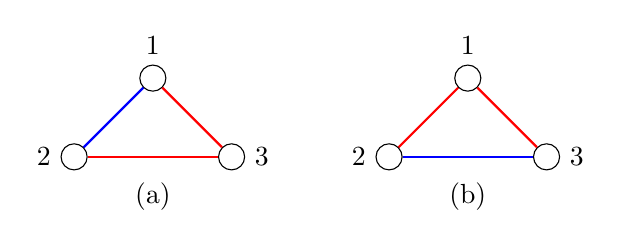
\begin{tikzpicture}
        \node[circle, draw, label={90:1}] (1a) at (0, 0) {};
        \node[circle, draw, label={180:2}] (2a) at (-1, -1) {};
        \node[circle, draw, label={0:3}] (3a) at (1, -1) {};
        \node at (0, -1.5) {(a)};

        \draw[thick, blue] (1a) to (2a);
        \draw[thick, red] (1a) to (3a);
        \draw[thick, red] (2a) to (3a);
        
        
        \node[circle, draw, label={90:1}] (1b) at (4, 0) {};
        \node[circle, draw, label={180:2}] (2b) at (3, -1) {};
        \node[circle, draw, label={0:3}] (3b) at (5, -1) {};
        \node at (4, -1.5) {(b)};
        
        \draw[thick, red] (1b) to (2b);
        \draw[thick, red] (1b) to (3b);
        \draw[thick, blue] (2b) to (3b);
    \end{tikzpicture}
\end{figure}
\noindent We can obtain (b) from (a) by rotating by $120^{\circ}$ anti-clockwise, so the two colourings essentially the same. Next, consider the following 2 triangles:
\begin{figure}[H]
    \centering
    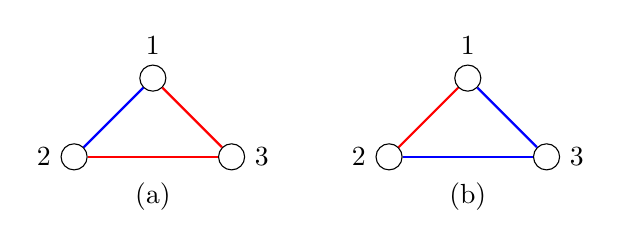
\begin{tikzpicture}
        \node[circle, draw, label={90:1}] (1a) at (0, 0) {};
        \node[circle, draw, label={180:2}] (2a) at (-1, -1) {};
        \node[circle, draw, label={0:3}] (3a) at (1, -1) {};
        \node at (0, -1.5) {(a)};

        \draw[thick, blue] (1a) to (2a);
        \draw[thick, red] (1a) to (3a);
        \draw[thick, red] (2a) to (3a);
        
        
        \node[circle, draw, label={90:1}] (1b) at (4, 0) {};
        \node[circle, draw, label={180:2}] (2b) at (3, -1) {};
        \node[circle, draw, label={0:3}] (3b) at (5, -1) {};
        \node at (4, -1.5) {(b)};
        
        \draw[thick, red] (1b) to (2b);
        \draw[thick, blue] (1b) to (3b);
        \draw[thick, blue] (2b) to (3b);
    \end{tikzpicture}
\end{figure}
\noindent It is not possible to rotate/reflect (a) to get (b) since (a) has one blue edge and (b) has two blue edges. So, the two colourings are essentially different. We can use Burnside's Lemma to count the number of essentially different symmetries. In this case, the group of symmetries of the triangle is $D_3$ and the set that it acts on is the set of colourings of the triangle $X$. We have 4 colours and 3 edges to colour, so $|X| = 4^3$. We consider now how many elements in $X$ each type of element in $G$ fixes:
\begin{itemize}
    \item The identity element $e$ fixes every element in $X$, so $X^e = X$.
    \item Now, consider the rotation element $r$. If a colouring $(a, b, c)$ is fixed by $r$, then $(a, b, c) = (b, c, a) = (c, a, b)$. Therefore, all 3 edges are coloured the same, i.e. we have only one choice to colour the triangle. So, $|X^r| = 4$.
    \item Finally, consider the reflection element $f$. If a colouring $(a, b, c)$ is fixed by $f$, then $(a, b, c) = (b, a, c)$. Therefore, two of the edges are coloured the same, i.e. we have only two choices to colour the triangle. So, $|X^f| = 4^2$.
\end{itemize}
\noindent In $D_3$, there is 1 identity element, 2 rotations and 3 reflections. So, Burnside's Lemma tells us that there are
\[|X/G| = \frac{1}{6} (4^3 + 2 \cdot 4 + 3 \cdot 4^2) = 20\]
essentially different colourings.

\newpage

\section{Semidirect Products}
We will now look at semidirect products. This generalise the concept of direct products. So, suppose that $G$ is a group, $H \leqslant G$ and $N \vartriangleleft N$ such that $N \cap H = \{e\}$ and $NH = G$, where
\[NH = \{nh \mid n \in N, h \in H\}.\]
Then, we say that $G$ is an (internal) semi-direct product of $N$ and $H$. These assumptions imply that there exists a bijection from $N \times H$ to $G$ via the map $(n, h) \mapsto nh$, but it need not be a homomorphism. Now, since $N$ is normal, we know that for all $h \in H$, $hnh^{-1} \in N$. Therefore, for $h \in H$, the map $\varphi_h: K \to K$ given by $\varphi_h(n) = hnh^{-1}$ defines an automorphism. For $n_1, n_2 \in N$,
\[\varphi_h(n_1n_2) = h(n_1n_2)h^{-1} = (hn_1h^{-1})(hn_2h^{-1}) = \varphi_h(n_1) \varphi_h(n_2),\]
so it is a homomorphism. Moreover, the map is bijective with inverse $n \mapsto h^{-1}nh$, i.e. $\varphi_h^{-1} = \varphi_{h^{-1}}$. Also, the function $\phi: H \to \operatorname{Aut}(N)$ given by $\phi(h) = \varphi_h$ is a group homomorphism.\sidefootnote{The group $\operatorname{Aut}(N)$ is the set of automorphisms of $N$, which forms a group under composition.} This is because, for $h_1, h_2 \in H, n \in N$,
\begin{align*}
    \phi(h_1h_2)(n) &= \varphi_{h_1h_2}(n) \\
    &= h_1h_2nh_2^{-1}h_1^{-1} \\
    &= h_1 \varphi_{h_2}(n) h_1^{-1} \\
    &= \varphi_{h_1}(\varphi_{h_2}(n)) \\
    &= \phi(h_1)(\phi(h_2)(n)),
\end{align*}
and so $\phi(h_1h_2) = \phi(h_1) \circ \phi(h_2)$. It turns out that the entire group structure of $G$ is determined by $N$, $H$ and $\phi$. If we have $g_1, g_2 \in G$, then since $G = HN$, $g_1 = h_1n_1$ and $g_2 = h_2n_2$ for $h_1, h_2 \in H$ and $n_1, n_2 \in N$. Moreover,
\[g_1g_2 = n_1h_1n_2h_2 = n_1(h_1n_2h_1^{-1})h_1h_2 = n_1 \varphi_{h_1}(n_2) h_1h_2.\]
Since $H$ and $N$ are known, we can multiply $n_1 \varphi_{h_1}(n_2)$ and $h_1h_2$, and similarly their product.

We will use this to define external semidirect product. Given two groups $N$ and $H$, and a group homomorphism $\phi: H \to \operatorname{Aut}(N)$, the external semidirect product of $N$ and $H$ with respect to $\phi$ (denoted by $N \rtimes H$ or $N \rtimes_{\phi} N$) is the set $N \times H$ with the operation
\[(n_1, h_1)(n_2, h_2) = (n_1 \phi(h_1)(n_2), h_1h_2).\]
If $G = N \rtimes_{\phi} H$ as above, then $N \times \{1\}$ forms a normal subgroup of $G$, and $\{1\} \times H$ forms a subgroup of $G$, and it need not be normal\sidefootnote{In fact, $H$ is normal if and only if $\phi$ is trivial.}. Moreover, $G$ is an internal semidirect product of these groups.

We now consider examples of semidirect products. Let $H$ and $N$ be groups. We can always take $\phi: H \to \operatorname{Aut}(N)$ to be the trivial homomorphism. In that case, for all $h \in H$, the map $\phi(h)$ is the identity map. Therefore, for $(n_1, h_1)(n_2, h_2) \in N \rtimes_{\phi} H$,
\[(n_1, h_1)(n_2, h_2) = (n_1 \phi(h_1)(n_2), h_1h_2) = (n_1n_2, h_1h_2).\]
So, this is the direct product of the groups $H$ and $N$. Now, let $n \in \mathbb{Z}_{\geqslant 3}$. The dihedral group
\[D_n = \langle r, f \mid r^n = 1 = f^2, frf = r^{-1}\]
is a semidirect product of the subgroup $N = \langle r \rangle$ and $H = \langle f \rangle$. The automorphism $\phi: H \to \operatorname{Aut}(N)$ is defined by $\phi_f = r \mapsto r^{-1}$.

We will now use group actions and semidirect products to classify all groups of order 15.
\begin{proposition}
Let $G$ be a group of order 15. Then, $G$ is cyclic.
\end{proposition}
\begin{proof}
By Cauchy's Theorem, we know that there exist $g_1, g_2 \in G$ such that $|g_1| = 3$ and $|g_2| = 5$. Let $H = \langle g_1 \rangle$ and $N = \langle g_2 \rangle$. Since $[G: N] = 3 < 5$, we know that $N$ is normal in $H$. By Lagrange's Theorem, we find that $H \cap N = \{e\}$.\sidefootnote{If an element is in their intersection, then its order has to divide both $|H| = 3$ and $|N| = 5$, i.e. its order is 1.} So, $NH$ is a subgroup of $G$. Moreover, since $H \leqslant NH$ and $N \leqslant NH$, we know that $NH$ has subgroups of order 3 and 5. By Lagrange's Theorem, this implies that $|NH| \geqslant 15$, and so $G = NH$. Therefore, there exists a homomorphism $\phi: H \to \operatorname{Aut}(N)$ such that $G \cong N \rtimes_{\phi} H$. We know that $N$ is a cyclic group of order 5, so the automorphism group $\operatorname{Aut}(N)$ is a cyclic group of order 4.\sidefootnote{Since $N$ is cyclic, a homomorphism $N \to N$ is determined by where it sends the generator $g_2$. We can send $g_2$ to any of the 5 elements in $N$ to give a different homomorphism- at the very least, they map the element $g_2$ to a different element in $N$. If we send $g_2$ to the identity, then the homomorphism is trivial. However, if we send $g_2$ to a non-identity element, the homomorphism cannot be trivial. By Lagrange, this implies that the image of the homomorphism is the entire group, i.e. it is an automorphism.} By the First Isomorphism Theorem, we know that $H/\ker (\phi) \cong \operatorname{Im}(\phi)$. So, we need $|\operatorname{Im}(\phi)|$ to divide $|H| = 3$. Moreover, since $\operatorname{Im}(\phi) \leqslant \operatorname{Aut}(N)$, we require $|\operatorname{Im}(\phi)|$ to divide $|\operatorname{Aut}(N)| = 4$. So, we must have $\operatorname{Im}(\phi) = \{id\}$, where $id$ is the identity permutation. This implies that 
\[g_1g_2g_1^{-1} = \phi(g_1)(g_2) = g_2,\]
meaning that $g_1$ and $g_2$ commute. So, $(g_1g_2)^n = g_1^n g_2^n$ for $n \in \mathbb{Z}_{\geqslant 1}$. In that case, $|g_1g_2| = \operatorname{lcm}(|g_1|, |g_2|) = \operatorname{lcm}(3, 5) = 15$. Therefore, $G$ is a cyclic group, generated by $g_1g_2$.
\end{proof}
\noindent Next, we classify all groups of order 21.
\begin{proposition}
Let $G$ be a group of order 21. Then, either $G$ is cyclic or $G$ has presentation
\[G = \langle g_1, g_2 \mid g_1^3 = g_2^7 = e, g_1g_2g_1^{-1} = g_2^2 \rangle.\]
In particular, there are 2 groups of order 21 up to isomorphism.
\end{proposition}
\begin{proof}
By Cauchy's Theorem, we know that there exist $g_1, g_2 \in G$ such that $|g_1| = 3$ and $|g_2| = 7$. Let $H = \langle g_1 \rangle$ and $N = \langle g_2 \rangle$. Since $[G: N] = 3 < 7$, we know that $N$ is normal in $H$. By Lagrange's Theorem, we know that $H \cap N = \{e\}$. So, $NH$ is a subgroup of $G$. Moreover, since $H \leqslant NH$ and $N \leqslant NH$, $NH$ has subgroups of order $3$ and $7$. By Lagrange's Theorem, this implies that $|NH| \geqslant 21$, and so $G = NH$. Therefore, there exists a homomorphism $\phi: H \to \operatorname{Aut}(N)$ such that $G \cong N \rtimes_{\phi} H$. We know that $N$ is a cyclic group of order 7, so the automorphism $\operatorname{Aut}(N)$ is a cyclic grouo of order 6. By the First Isomorphism Theorem, we know that $H/\ker (\phi) \cong \operatorname{Im}(\phi)$. So, we need $|\operatorname{Im}(\phi)|$ to divide $|H| = 3$. Moreover, since $\operatorname{Im}(\phi) \leqslant \operatorname{Aut}(N)$, we need $|\operatorname{Im}(\phi)|$ to divide $|\operatorname{Aut}(N)| = 6$. So, either $|\operatorname{Im}(\phi)| = 1$ or $|\operatorname{Im}(\phi)| = 1$. We consider each case separately:
\begin{itemize}
    \item First, assume that $|\operatorname{Im}(\phi)| = 1$. Then, we must have $\operatorname{Im}(\phi) = \{id\}$, where $id$ is the identity permutation. This implies that 
    \[g_1g_2g_1^{-1} = \phi(g_1)(g_2) = g_2,\]
    meaning that $g_1$ and $g_2$ commute. So, $(g_1g_2)^n = g_1^n g_2^n$ for $n \in \mathbb{Z}_{\geqslant 1}$. In that case, $|g_1g_2| = \operatorname{lcm}(|g_1|, |g_2|) = \operatorname{lcm}(3, 7) = 21$. Therefore, $G$ is a cyclic group, generated by $g_1g_2$.
    
    \item Now, assume that $|\operatorname{Im}(\phi)| = 3$. Then, we must have $\operatorname{Im}(\phi) = \{id, \sigma, \sigma^2\}$, where $\sigma(g_2) = g_2^2$.\sidefootnote{The automorphism $\sigma$, given by $g_2 \mapsto g_2^2$ has order 3, since $\sigma^3(g_2) = \sigma^2(g_2^2) = \sigma(g_2^4) = g_2^8 = g_2$. Also, since $\operatorname{Aut}(N)$ is cyclic, we know that this is the only subgroup of order 3.} So, we can have $\phi(g_1) = \sigma$ or $\phi(g_1) = \sigma^2$. If $\phi(g_1) = \sigma$, then we have
    \[g_1g_2g_1^{-1} = \phi(g_1)(g_2) = \sigma(g_2) = g_2^2.\]
    This gives us the presentation
    \[G = \langle g_1, g_2 \mid g_1^3 = g_2^7 = e, g_1g_2g_1^{-1} = g_2^2 \rangle.\]
    Instead, if $\phi(g_1) = \sigma^2$, and so $\phi(g_1^{-1}) = \sigma$. So, we have
    \[g_1^{-1} (g_2) g_1 = \phi(g_1^{-1})(g_2) = \sigma(g_2^2) = g_2^2.\]
    This gives us the presentation
    \[G = \langle g_1^{-1}, g_2^2 \mid (g_1^{-1})^3 = (g_2^2)^7 = e, g_1^{-1} (g_2^2) g_1 = g_2 \rangle.\]
    Therefore, the two presentations give rise to isomorphic groups.
\end{itemize}
So, there are exactly 2 groups of order 21, up to isomorphism.
\end{proof}

\end{document}
